\documentclass[a4paper,oneside]{report}

\usepackage{amsmath}
\usepackage{amssymb}
\usepackage[english]{babel}
\usepackage{fancyhdr} 
\usepackage{multirow}
\usepackage[pdftex]{graphicx}
\usepackage{listings}      
\usepackage{pdfpages}
\usepackage{setspace}
\usepackage{url}

\makeatletter


%
% Some custom definitions
%

% add horizontal lines
\newcommand{\HRule}{\rule{\linewidth}{0.5mm}}
\newcommand{\HRuleLight}{\rule{\linewidth}{0.1mm}}

% custom part page
\def\part#1#2
{
	\par\break
  	\addcontentsline{toc}{part}{#1}
	\noindent
	\null	
	\HRuleLight\\[0.0cm]
	\vspace{20pt}	 
	\begin{flushright} 		
  	{\Huge \bfseries \noindent #1}\\
  	\vspace{30pt} 
	\begin{minipage}{0.85\textwidth}
		\begin{flushright}
		{\large \noindent #2}
		\end{flushright}
	\end{minipage}\\[0.75cm] 
	\end{flushright} 		
	\thispagestyle{empty}
	\break
}

% chapter header
\renewcommand{\@makechapterhead}[1]
{\vspace*{50\p@}{
	\parindent \z@ \raggedright \normalfont
	%\huge \bfseries \thechapter. #1
	\huge \bfseries #1
	\vspace{20pt}}}

\setcounter{secnumdepth}{-1} 
\onehalfspace
\oddsidemargin 1in 
\oddsidemargin 0.6in 
\topmargin -0.3in
\setlength{\textwidth}{14cm}
\setlength{\textheight}{23cm}
\lstset{language=C} 

\begin{document}

%
% Cover page
%
\begin{titlepage}
\begin{center}


\includegraphics[width=120mm]{sources/images/cogito_logo_main.png}

\HRuleLight\\[0.5cm]

\begin{minipage}{0.45\textwidth}
	\begin{flushleft}\large
		\emph{Author:}\\
			\textbf{Thomas \textsc{Taylor}}\\[0.27cm]
			Computer Science (Games)
			Student Number: 08813043
	\end{flushleft}
\end{minipage}
\begin{minipage}{0.43\textwidth}
	\begin{flushright} \large
		\emph{Supervisor:} \\
		\textbf{Graham \textsc{Winstanley}}\\[0.25cm]
		\emph{Second Reader:}\\
		\textbf{Saeed \textsc{Malekshahi}}
	\end{flushright}
\end{minipage}\\[0.75cm] 

\HRuleLight\\[0.2cm]

\large School of Computing, Engineering and Mathematics\\ \textbf{University of Brighton}

\vfill
\huge Project Documentation\\
\large April, 2012\\

\end{center}
\end{titlepage}



%
% Table of contents
%
{
	\renewcommand\thepage{}
	\setcounter{tocdepth}{1}
	\tableofcontents
	\clearpage
}

% reset page count
\setcounter{page}{1}


%
% Start of content
%

\chapter{Introduction}

The artificial intelligence (AI) techniques used by game developers are often called archaic by academic AI researchers, which may indeed be true, however, it is important to view such techniques in the context of which they are used. While academic AI researchers are able to use as much processing power as the hardware can afford them, game developers are much more limited, having to compromise with other processes such as physics, sound, networking and most importantly the graphics processing. For this reason, it is more understandable that game developers squeeze as much functionality as possible using minimal processor time (the A* search algorithm is still one of the most popular AI algorithms used in games today, and was first introduced over 30 years ago). Indeed, modern game AI programming is more a skill of employing the cheapest (computationally) techniques, and often means that shortcuts and workarounds are a necessity in order to achieve `believable' AI. 

That being said, we are starting to see a change taking place in the computer games industry which suggests that the processing time availiable for often overlooked processes such as AI is starting to increase. One such factor in this change is the so-called `graphics plateau'. It has been said that we have reached an `acceptable' level of graphical complexity whereby we are unlikely to see any more major advances in the field, but rather `iterations' \cite{Sheffield:2008fk}. Given the rate of hardware advancement, we are sure to see much more processor time freed up for those processes such as AI which have been treated as `extraneous' in the past. 

Another important factor in this change is the emergence of the `casual' gamer. With casual games now accounting for a considerable proportion game sales, the consumer has shown that there is a big market for games which have less emphasis on complex graphics effects, and more emphasis on interesting gameplay mechanics \cite{Association:2011uq}. Indeed, with Nintendo's Wii home console having far outsold both Sony's PlayStation 3 and Microsoft's Xbox, the consumer has shown that they value unique gameplay and accessibility over advanced graphics \cite{:2012dq, Nintendo:2012nx, :cr}. 

With these factors already starting to bring about a change in the priority that developers give to the components of their games, I believe that now is as good a time as any for developers to introduce some more advanced AI techniques into their games.

\section{Project Aims and Objectives}

The main aim of my project was to experiment with some more advanced academic AI techniques which are not typically found in commercial games, and look into whether such techniques were viable with today's hardware. This second point is key, especially given the popularity of `limited' hardware such as the Nintendo Wii, and mobile devices.

The sub-field of AI that I chose to focus my project on was machine learning, as it is an emerging field which greatly interests me and one which I feel is a natural fit for computer games, and one we could see utilised in many forms in future games.

For my project, I wanted to develop an AI system which was capable of employing machine learning techniques in order for a number of AI-controlled agents to safely navigate a 2D game environment. I wanted the agents to be able to develop a knowledgebase dynamically, with no need for prior training, or knowledge of the game world. I then wanted the agents to be able to apply this gained knowledge in order to hopefully increase their chances of survival. 

\section{Background}

I chose the classic Commodore Amiga game `Lemmings' as the context and main inspiration for my project.

\begin{figure}[h!]
  \centering
    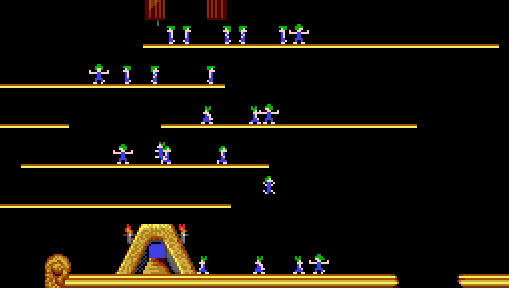
\includegraphics[width=100mm]{sources/images/lemmings3}
    \caption{A typical level in Lemmings.\label{screen}}
\end{figure}

Originally released in 1991 for the PC and Commodore Amiga, `Lemmings' has a very simple premise: to guide a group of computer-controlled `lemmings’ across a level from the entrance-point to the exit. The Lemming characters themselves have very basic AI; capable of merely walking across the level map. The level itself consists of a number of platforms, along with a number of hazards which will kill the Lemmings (big drops, pits etc.). The goal of the player is to utilise a set of tools in order to ensure that the Lemmings safely reach the level exit, such as umbrellas for big drops, girders to cross pits etc. 

For my project, I planned to take this concept, simplify it by removing some of the tools and obstacles, and program some AI agents to learn for themselves how to best traverse the level, without any human interation.
		
\section{The Project in Context}
	
Throughout the development of my project, I needed to utilise skills which I had gained from modules I had studied during my course.

There was obviously a lot of knowledge that I gained in the AI-related modules I have studied (CI213 - Intelligent Systems and CI342 - Advanced AI) which I could directly apply to my project. Techniques such as pathfinding algorithms, and generally approaching AI-based problems from an academic angle.

I was also able to apply a lot of useful knowledge that I had gained from the programming-based modules from my course (CI101 - Introduction to Programming, CI228 - Object-Oriented Software Design and Specification and CI346 - Programming, Concurrency and Client-Server Computing). I applied a lot of the `good' object-oriented design practices which were learnt in these modules: principles such as inheritance and design patterns like the singleton. I also found the knowledge learnt this year in CI346 very useful to overcome some concurrency issues I had using multiple threads in my system.

Another module I have found to be very useful is CI224 (Games Development). Many of the game design concepts: physics, object transformations, model loading, and various other useful skills. The project we did in CI224 was particularly useful, as it introduced me to the process involved in developing a game from scratch. I was also introduced to source control systems in CI224, which has proven to be invaluable knowledge to have.

I also used the knowledge of object-oriented software design and UML learnt in CI228 and CI231 (Formal Underpinnings and Specification) to design my system. Although I didn't actually use the formal specification language learnt in my system specification, I could still apply the concepts learnt to my own designs.

I learnt a great deal about data access and performance optimisation in the CI312 (Computer Graphics Algorithms) module. It really helped me too look at my code at a lower level, and analyse the best and most efficient ways to access and manipulate data; something which I have found to be incredibly important, especially in a game context, where some functions can be called 60 times every second. This is something which is of paramount importance, especially in games, as you will likely be carrying out certain functions up to 60 times every second, so any inefficient code would cause big problems in performance. 



%
% New part
%

\part{Research}{This section documents the research that I carried out prior to designing my system, and how it influenced my final designs. \\ \ \\The section is split into two subsections: my research into AI, and my research into the more game-related topics.}

\chapter{Artificial Intelligence}

Since the early days of computing, computer scientists have striven to replicate in machines the defining characteristic that makes us human: intelligence. One of the first references to `intelligent machines' came in 1950 in Alan Turing's seminal paper \emph{Computing Machinery and Intelligence}, in which Turing opens with the words: "I propose to consider the question, 'Can machines think?'". In it, he outlines a test in which a human participant engages in conversation with a machine designed to imitate human behaviour, known as the Turing Test. This paper also inspired us to look philosophically at what it is that makes us inherently human, and whether this is indeed replicable in a machine.

The term `artificial intelligence' was later formally defined in 1955 by McCarthy et al in the proposal for the Dartmouth Summer Research Conference on Artificial Intelligence, which is considered by many to be the origin of the field of AI \cite{Crevier:1993kl}. In the proposal, it was suggested that ``every aspect of learning or any other feature of intelligence can in principle be so precisely described that a machine can be made to simulate it" \cite{McCarthy:1955ve}. Since these early days, the field of AI has grown to become an integral field not only in computer science, but also in the infrastructure of every industry \cite{Kurzweil:2005ly}. 

\section{AI In Games}

One area where AI techniques are used extensively is computer games. Whether to map a route across obstacle-ridden terrain, control the actions of non-player characters (NPCs) or even to adjust game parameters to fit to the skill of the player, AI plays a key role in almost all modern computer games. However, due to the nature of the final product, game AI takes a very contrasting approach to that of academic AI. While the aim with academic systems is always to provide the most complete and accurate results, the ultimate aim with game AI is to provide entertainment for the user by giving the illusion of intelligence. Ironically, this can often mean that it is necessary to make the system intentionally `stupid' by building flaws in the system or even by allowing the system to cheat to ensure that the game AI behaves `realistically' \cite{Liden:2004fk}. Additionally, academic AI systems usually have very simplistic visualisation, allowing the majority of processing time to be dedicated to the AI. Game AI on the other hand, must run simultaneously with a number of other processes such as the physics engine, sound and most significantly graphics which in reality means that the AI processing is often compromised in the favour of other processes. In the proceeding sections, I outline some of the most popular AI techniques used in commercial computer games today.

\subsection{Finite State Machines} 

Finite state machines (FSMs) are one of the most commonly used AI techniques found in games today. As the name suggests, FSMs are ``simple, rule-based systems in which a finite number of 'states' are connected in a directed graph by 'transitions' between states" \cite{:hc}. One of the first games to sucessfully use FSMs was Atari's 1979 game \emph{Pacman}, in which the enemy ghost characters use a FSM to define states (chase, run away and roam), changing their state in response to in-game triggers. FSMs are used extensively in many commercial games, as they are relatively easy to understand, implement and debug \cite{Bourg:2004tg}.

\subsection{Search and Planning Systems} 

Search systems are primarily concerned with finding actions/states in a graph to satisfy a goal condition (or at least to get as close as possible). Planning systems are a specific branch of search which have an emphasis on finding the best (or simplest) sequence of actions required in order to reach the goal state. Many algorithms have been developed, but the A* algorithm is the one used most extensively, due to its performance and the accuracy of its results. Search and planning systems are used for a variety of tasks, from the pathfinding of AI agents in a first-person shooter game to the allocation of resources in a real-time strategy game. Blizzard's 1994 game \emph{Warcraft} is an example of an early implementation of using the A* pathfinding algorithm to navigate agents.

\subsection{Artificial Life} 

An artificial life (A-life) system is designed to exhibit realistic and lifelike behavior in game characters. A-life systems are often used to coordinate the movement of multi-agent systems to make the agents maneuver in flock and herd formation. One of the most compelling reasons to use A-life techniques is that more complex behaviours can emerge as a result from the pre-programmed rules \cite{Woodcock:bs}. \emph{The Sims} developed by Maxis (now part of EA) is probably one of the best known games to use A-life techniques, and uses so-called `smart terrain' to broadcast information to the game characters. For example, a hungry character may walk past a refridgerator, which broadcasts that it contains food. After collecting the food, the nearby oven broadcasts that it can cook the food, leading the character to it \cite{Woodcock:bs}. These individual object-level actions when combined, cause the character to exhibit realistic `emergent' behaviour which, while very useful, is also incredibly difficult to debug. Additionally, the techniques can be incredibly processor intensive, making them unsuitable for some games. 

\subsection{Scripting} 

Another popular technique in game AI is scripting, whereby developers use a specialised high-level scripting language to outline the NPCs reactions to basic situations and hard-code game events. Scripting allows the game engine to be accessed externally in a safe `sandbox' environment, greatly reducing the chance of bugs and errors, so is suitable for non-programmers such as designers. For this reason, there is a large community of gamers who use scripting interfaces to create additional game content. Lionhead Studios used scripting heavily in their 2001 game \emph{Black \& White} to present the game's storyline using a series of in-game challenges rather than more traditional cut-scenes \cite{:hc}. A big disadvantage to using scripting is that it requires every character behaviour and game scenario to be hard-coded which is incredibly time consuming for the programmer/developer, and is not always possible. Additionally, using scripting can be very restrictive for the player, as the story progression is often very linear.

\subsection{Cheating The System}

Game developers also use a number of hacks and workarounds to give their AI systems the illusion of intelligence while retaining the entertainment value; in many cases, traditional AI techniques are unnecessary. In computer games, entertainment is paramount, and so it may be inappropriate to implement a very `smart' adaptive AI system. Consider Konami's stealth-action series \emph{Metal Gear Solid} in which the player must navigate a level while avoiding detection from the guard NPCs. Using a truly intelligent and adaptive AI system would remove a lot of the entertainment value of the game which in which the player must recognise patterns in guard behaviour in order to progress. While this AI system would be considered flawed in the eyes of an academic researcher, it is perfectly acceptable (even preferable) in the context of the game. Game developers also afford the AI system extra information or resources unavailable to the player. This is particularly useful in real-time strategy games to give the computer access to extra troops or supplies. Using these kinds of `cheats' can be an acceptable way to increase the level of difficulty, although it can be a challenge to disguise this from the player. If the player feels that the game is acting unfairly and that their actions are ineffective, they will obviously not enjoy the game.

\subsection{The Future of Game AI}

From as early as 2000, statistics were showing that the industry was beginning to take AI more seriously. Figures collected from the AI roundtable at the annual Game Developer's Conference showed that not only were a lot more studios employing dedicated AI programmers, but that the average amount of CPU time reserved for AI processing increased from 5\% to over 25\% \cite{Woodcock:oq}.

\section{Machine Learning}

\begin{quotation}``A computer is said to learn from experience \emph{E} with respect to some class of tasks \emph{T} and performance measure \emph{P}, if its performance at tasks in \emph{T}, as measured by \emph{P}, improves with experience \emph{E}." - \textbf{Tom Mitchell} \cite{mitchell1997machine} 
\end{quotation}

The ability to learn is one of the central features of intelligence \cite{Langley:1996zr}. To then apply this knowledge and modify behaviour accordingly when faced with similar scenarios is an area which has recieved a considerable amount of research. In fact, machine learning techniques are already in use in a number of commercial applications such as speech recognition, robotic control and machine vision, proving that it can be a very useful solution, especially in solving problems which may have unexpected outcomes that cannot be predicted by the software developer.

\paragraph{Online and Offline:} Learning which takes place while a system is running is said to be `online', while `offline' learning refers to a system which modifies its behaviour \emph{after} it has finished running. Whilst online learning provides instantaneous results, it also makes the system much more difficult to debug were any issues found, due to its continous modification.

\paragraph{Supervised and Unsupervised:} Learning which utilises example training data is described as `supervised', whereas a system which only has access to the data that it collects itself is described as `unsupervised'. The benefit to supervised learning is that the system can base its learning on some correct `solutions', which lead to more accurate and perhaps `quicker' learning. However, the training data itself needs to be collected and analysed, which requires human input, and can become very time consuming. Unsupervised methods on the other hand do not have this requirement, but must analyse the collected data to find hidden structure; there is no `correctness' indicator to evaluate potential solutions. There are also techniques which form an intermediary between the two, using both labelled and unlabelled data. These methods are known as `semi-supervised'.

\subsection{Reinforcement Learning}

Reinforcement learning (RL) is the name given to the subset of machine learning techniques which use a reward system to let the system know how it is performing. The overall aim of RL being to maximise the cumulative reward. RL uses a cause and effect loop whereby the system begins in a state, performs an action (recieving a reward), which causes the environment to change its state, repeating the cycle (see Figure 2).

\begin{figure}[h!]
  \centering
    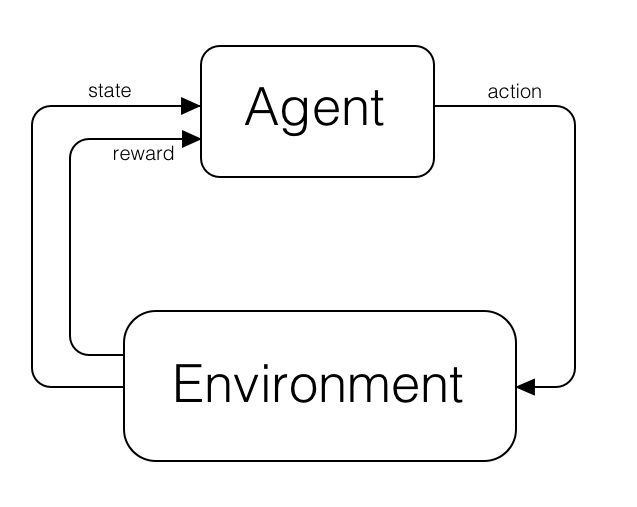
\includegraphics[width=70mm]{sources/images/RLDiagram}
    \caption{The Reinforcement Learning Loop \cite{Nilsson:2010qa}.\label{screen}}
\end{figure}

What sets RL apart from other types (supervised/unsupervised methods) is that the learner is never given correct input/output, nor are any incorrect actions ever corrected, leaving the system to deduce where an error has occurred. This can be particularly tricky to ascertain as an error can often occur due to a poor decision made several timesteps in the past. Similarly, the mistake could have been made as a result of 20 previous actions, all of which would have to be repeated in sequence to replicate the error. This is known as the `credit assignment problem', and results from the fact that RL uses a sequential style of learning, where a system makes many decisions which lead to an eventual goal condition. In an attempt to combat this, RL introduces the notion of `regret', by taking into account the long-term effects of actions. For example, an RL system may choose an action with a negative immediate reward so as to maximise its long-term reward. RL also involves finding an acceptable compromise between exploration (of new undiscovered terrain) and exploitation (of the system's current knowledgebase).

RL algorithms are split into two main categories: dynamic-programming-based (which themselves are not strictly RL), and the `truly' RL algorithms. Which algorithms can be used depends on the information we have about the environment. If the state transition probabilities and the reward functions for the environment are already known, we can calculate the optimal policies using standard dynamic-programming techniques such as value-iteration and policy-iteration. First described by Richard Bellman, dynamic programming aims to solve problems by simplifying them into subproblems and solving those recursively. If on the other hand, we do not know state transition probabilities, the policy must be learned using `true' RL algorithms such as Q-learning.

\subsubsection{Markov Decision Processes:}

Markov decision processes (MDPs) are often used to model the environment in which the system is intended to be used. An MDP is usually represented as: $MDP(S, A, \{Psa\}, \gamma, R)$ and consists of 5 main components: 

\begin{enumerate}
	\item A set of possible states \emph{S}
	\item A set of available actions \emph{A}
	\item Probability \emph{P} of moving from the current state \emph{s} to a new state \emph{$s^\prime$} by taking action \emph{a}
	\item The discount factor $\gamma$ where 0 $\leq \gamma \leq$ 1 (adjusts the influence of future rewards)
	\item A reward function \emph{R}, which maps from a state to a real number $R : S \mapsto \mathbb{R}$ 
\end{enumerate}

\subsubsection{The Theory} 

In order for the algorithms to compute an optimum policy, the system must first build up a knowledgebase through experience. It does this simply by executing:

\begin{enumerate}
	\item Starting in state $s_0$, it performs action $a_0$ (often chosen at random during this learning phase), causing the system to move to a new state $s_1$ according to the probability function for $s_0$ and $a_0$ which may or may not be necessary (e.g. a robot may have an inaccurate direction sensor, which when set to move north, causes it to move north 80\% of the time, with a 10\% of going east, and a 10\% chance of going west).
	\item After running for an amount of time, the system will have reached a number of states ($s_0, s_1, s_2, s_3 ...$) The performance of the system can then be evaluated using a reward function, whereby the cumulative rewards would be: $R(s_0) + R(s_1) + R(s_2) + R(s_3) + ...$
	\item The final step is to factor in a discount factor, which gives us: $R(s_0) + \gamma R(s_1) + \gamma^2 R(s_2) + \gamma^3 R(s_3) + ...$ (Whereby the reward received at timestep $t$ is discounted by $\gamma^t$, which gives a greater weighting to rewards now than to rewards in the future).
\end{enumerate}

The ultimate goal of the RL algorithm is to formulate a policy\footnote{The term `policy' is used to refer to a set of action/state mappings often symbolised by $\pi$} which maps states to actions ($\pi: S \mapsto A$) such that for every state, the policy recommends the optimum action to take. After a certain number of iterations of the algorithm, the policy's values become static (i.e. they are no longer updated). This signifies that the optimum policy has been found, and the values have \emph{converged}. This could take as little as a few thousand iterations for small problems, but more likely will take many more. In many real-world cases, there may not be enough time to reach convergence, in which case the best policy would be used.

\subsubsection{Algorithms}

There have been a variety of different RL algorithms developed, each with their own advantages and disadvantages. There have been many algorithms developed to perform RL, including Temporal Difference, Monte Carlo, Bucket Brigade and Q-learning which is described in more detail below.

\subsubsection{Q-learning}

Originally proposed by Christopher Watkins in 1989 \cite{Watkins:1989mi}, Q-learning takes a slightly different approach to other RL algorithms, as it doesn't require a complete model of the environment, which can be a big advantage in certain scenarios, as it is not often not possible (or indeed feasible) to generate a model before the system has run. Q-learning gets its name from the quality information, or Q-values which it stores for each state-action pair. This Q-value represents how `good' the system thinks that an action is to take when in a given state.

\noindent The Q-learning algorithm is as follows:
\begin{equation*}
	Q(s_t,a_t) \Leftarrow Q(s_t, a_t) + \alpha_t(s_t, a_t)[R(s_t) + \gamma max_{a_{t+1}} Q(s_{t+1}, a_{t+1}) - Q(s_t, a_t)]
\end{equation*}

\noindent But is often rewritten more simply as:
\begin{equation*}
	Q(s_t,a_t) \Leftarrow Q(s_t, a_t) + (1 -\alpha_t) + \alpha[R(s_t) + \gamma max Q(s_{t+1}, a_{t+1})]
\end{equation*}

Where $Q(s_t, a_t)$ represents the Q-value for the current state/action, $R(s_t)$ represents the reward associated with the current state and $max Q(s_{t+1}, a_{t+1})$ represents the maximum possible Q-value for the next state. Q-learning also introduces and addition variable known as the learning rate (represented as $\gamma$), which affects how quickly the Q-values are modified; a greater learning rate results in much faster changes to Q-values. It is common practice to begin with a large learning rate, and decrease it as time goes on, to fine-tune the Q-values. Researchers at Tel-Aviv University carried out some interesting research into the effect of learning rates on the rate of convergence, which suggests that convergence can be reached much quicker if using a variable learning rate.

Updating the old Q-values ensures that the system retains all previously obtained knowledge. Introducing the max Q-value into the equation means that the success (or failure) of an action is reflected in earlier actions, in effect `trickling' back up the supply chain.

Q-learning converges with probability 1, meaning that after sufficient iterations of the algorithm, the learner will have formulated an optimal policy such that they can move towards the most desirable state from any other state.

\subsection{Decision Tree}

Another popular type of machine learning is Decision Tree Learning. Decision Tree Learning approaches problem solving using classification to label input data. A tree structure is used to do this, with each node representing tests and the leaf nodes representing categories (leaf nodes can also represent numerical values). Each of these tests serve the function of sorting the input data; as the data moves down the tree, it will eventually filter through to a leaf (or category) node. The tests can be multivariate (where multiple attributes are tested at once), or univariate (where only a single attribute is tested). The outcomes to each test must be mutually exclusive. 

When building a decision tree, the ultimate goal is to order the tests in the tree in such a way that each level gives the maximum reduction in the entropy (or uncertainty). This is known as uncertainty reduction. There have been various algorithms developed to construct decision trees, the majority of which use a top-down approach. Among these are the ID3 and C4.5 algorithms (both developed by Ross Quinlan), and CART (developed by Leo Breiman et al) \cite{Quinlan86inductionof,Quinlan:1993:CPM:152181,breiman1984classification}.

One of the main benefits to using decision trees is that they are relatively easy to use and understand; decision trees are easy to visualise and read. Another key advantage is that tree structures are very commonly used in computer science, and so there exist various highly optimised algorithms for the building and searching of trees.

However, decision trees can lack accuracy; the size of the tree will increase tremendously if a much higher resolution output is required \cite{schwab2004ai}. Additionally, decisions trees do not scale well, with very large, highly complex trees being very difficult to maintain. Another important point to mention is that because game AI systems are required to learn online as the game is played, supervised techniques such as back propagation are inappropriate. Another issue related to decision trees is that of replicated subtrees (see Figure 3).

\begin{figure}[h!]
	\centering
		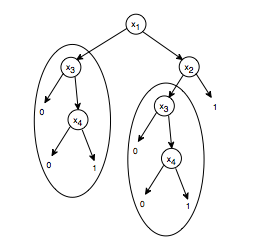
\includegraphics[width=60mm]{sources/images/ReplicatedSubtrees}
    	\caption{Replicated Subtrees}
\end{figure}

\subsection{Genetic Algorithms}

Another popular type of machine learning is the 

Pros:
\begin{itemize}
	\item When it may be too computationally expensive to calcuate a decision
	\item To complement other AI techniques
	\item Relatively simple to set up and start getting results, even if you don't know how to solve the problem otherwise
\end{itemize}

\noindent Cons:
\begin{itemize} 
	\item Evolution is often time-consuming, taking many generations
	\item Not guaranteed to find an optimal or even satisfactory solution
	\item Don't cope well with components which may not have a concrete design; the addition of features can require a complete redesign of the genetic algorithm
\end{itemize}

\subsection{Artificial Neural networks}

Artificial Neural Networks (ANNs) are another popular machine learning technique which are inspired by the neural networks found in the brain. ANNs consist of a group of interconnected nodes (or neurons)

An artificial Neural Network (NN) is an electronic simulation based on a simplified human brain. In an NN, knowledge is acquired from the environment through a learning process and the network’s connection strengths are used to store the acquired knowledge [20].

An NN can be used to make decisions or interpret data based on previous input and output it has been given. The important difference is that the current state doesn’t need to have been hard-coded. Instead, the NN makes the best approximation that it can, based on the states that it already knows about. This means that the NN will choose an action that would have been performed in a similar state.

So far, game developers have been reluctant to allow a game to ship `active' learning in case the AI were to learn something stupid.

Some examples of applications that NNs are being used for are predicting sales, handwritten character recognition for PDAs and faxes, odour analysis via electronic nose, stock market forecasting, credit card fraud detection, Pap smear diagnosis, protein analysis for drug development and weather forecasting. 

This technique’s flexibility means that it has the potential to be applied in a wide range of situations in future games. Therefore, it is likely that NNs will play a bigger role in commercial games in the near future.

\subsection{Applications For Machine Learning}

While it has yet to be utilised prominently in the game industry, machine learning is already used effectively in many other application areas. Tom Mitchell outlines current application areas for machine learning in his 2006 article \emph{The Discipline of Machine Learning} \cite{Mitchell:2006fv}:

\paragraph{Speech recognition:} All commercial systems currently available use machine learning to train the system. Many use a two-phase learning method: an initial phase for general learning carried out prior to the product being shipped, and a second phase which takes place post-purchase and tunes the system to the customer.

\paragraph{Computer vision:} Many of the currently available vision systems utilise machine learning techniques. One of the largest scale vision systems is in use by the US postal service to sort letters with hand-written addresses, and sorts over 85\% of handwritten mail in the US.

\paragraph{Robot control:} Much research has gone into training robotic systems using machine learning. Researchers at Stanford University have demonstrated a system capable of advanced helicopter flight \cite{Ng:2004dz, Abbeel07anapplication, Abbeel:fu}. This type of system could be very useful in space exploration.

\paragraph{Accelerating empirical sciences} Machine learning is also being used to aid in scientific discovery, such as gene analysis, in the field of astronomy for sky surveillance and to analyse brain activity. Machine learning methods are particularly useful in data-intensive areas.

\subsection{Machine Learning In Games}

As discussed, machine learning techniques have been integrated into many different areas of computer science and indeed many other fields. Such techniques have yet to reach the same kind of penetration in the computer game industry. That being said, a fair amount of research has been conducted by the academic community into the appliation of machine learning in a computer game environment. 

\subsubsection{Academic Examples}

Machine learning techniques were first applied to board games such as checkers \cite{Samuel:1959qo, Samuel:1967ye}. In 2002, researchers David Fogel and Kumar Chellapilla created an evolutionary algorithm using neural networks to develop a checkers-playing system capable of beating its creators after just 10 generations \cite{Fogel:2003fk}. After 840 generations and 165 games, the system reached an `expert' level on a competitive online checkers website, placing it in the top 500 of the 120,000 players on the site. While this is impressive, most board games emphasise only a few human capabilities such as search and decision-making \cite{Laird:2001tw}. 

In 2005, researchers at the University of Texas developed a reinforcement learning system called rtNEAT capable of learning in real-time using neural networks \cite{Stanley:2005ff}. Rather than simply playing games, the system is trained by the player, who sets up training exercises using various objects and obstacles. Additionally, the player can adjust the algorithm's coefficients for fitness components using a number of slider interface elements, allowing the player to determine `ideal' behaviour. The player can adjust how the AI characters disperse, use cover or approach enemies for example. This technique is particularly interesting as it allows the player to directly train the system themelves. Giving this kind of control and customisability over the AI's learning could be an attractive feature to players. 

In another example, researchers at the university of Maastricht conducted a number of experiments into a reinforcement learning-based `dynamic scripting' which uses ``an adaptive rule-base for the generation of game AI on the fly" \cite{Spronck:2005fu}. The experiments showed that after just 25 games, the dynamically scripted AI was able to develop a strategy to outperform the static AI for at least 10 consecutive encounters. This technique could be an attractive alternative to other machine learning techniques as it allows dynamic adaptive behaviours, while still allowing the developers to script certain behaviours, allowing more control than is typically possible with other methods.

A research group led by Robin Baumgarten developed an approach for ``simulating human game-play" using a variety of techniques built upon Introversion Software's 2006 strategy game \emph{DEFCON} \cite{Baumgarten:2008il}. The system displays an impressive level of intelligence through its planning of fleet movements and attacks as well as more low-level such as coordinating bombing runs and assigning bombing targets. To do this, the system maintains a knowledgebase of past games, which it uses to generate a plan for the current situation using a decision tree-based method. The system proved effective, with the system beating the static AI system in 76.7\% of games. Most interesting about the research is the survey they conducted (albeit with a group size of 10 which is too small to be statistically significant). The results of the survey showed that the more advanced AI system was less popular with novice players, who felt a greater level of frustration and therefore less desire to play again. This is an interesting point, as it demonstrates the differences between academic and game AI; while it may seem important to an academic researcher to develop a very strong adaptive AI system, the player would not necessarily show the same kind of enthusiasm.

\subsubsection{Commercial Examples}

Despite the promising academic research over the last decade, few commercial developers have used machine learning in their games. One of the few commercial games to employ such techniques to real effect was Lionhead Studios' god game \emph{Black \& White} \cite{:hc}. In \emph{Black \& White}, the player becomes a deity tasked with watching over a group of followers. Over the course of the game, the player must recruit as many followers as possible in order to gain influence over the land. To aid with this task, the player is given an AI controlled `creature', which the player must train to do his bidding. Lionhead implemented this learning using an approach they call `representational promiscuity', which is based on the idea that no single method could be used to build a complete agent. The creatures use a `Belief-Desire-Opinion-Intention' architecture to represent the creature's knowledge about the environment. When the creature percieves information in its environment, it is stored in memory as a `belief'. The creature uses these beliefs to form opinions which alter their desires in-game to suit the player. To form opinions about its environment, the creature builds decision trees by looking at attributes that best categorise the knowledge into groups (see Figure 4 for an example).

\begin{figure}[h!]
	\centering
		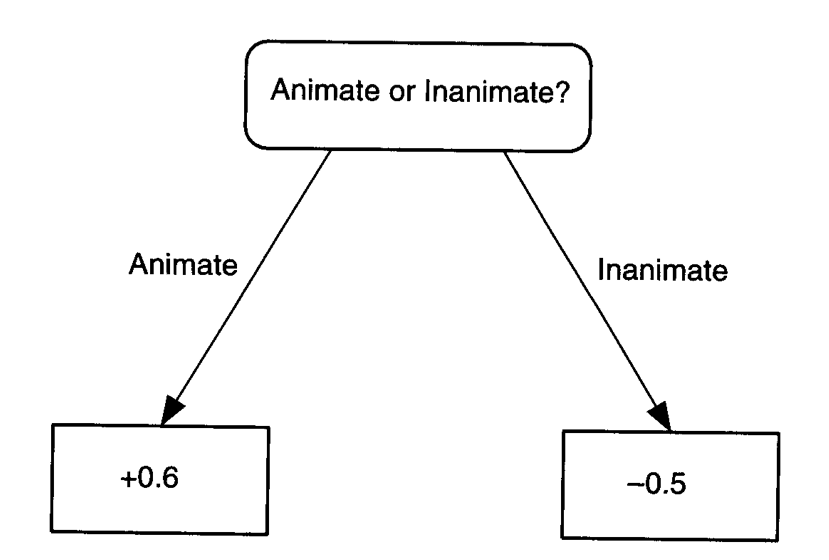
\includegraphics[width=80mm]{sources/images/TastyTree}\paragraph{}
    	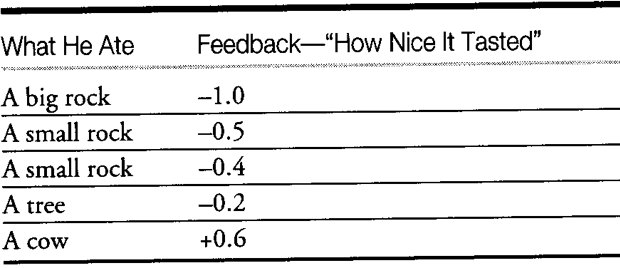
\includegraphics[width=80mm]{sources/images/TastyTable}
    	\caption{An example decision tree generated from the creature's experience eating objects \cite{:hc}.}
\end{figure}

From these trees, a creature is able to make a prediction as to the outcome of performing a certain action. In the case of the example above, the creature would deduce that inanimate objects taste worse than animate ones, making it less likely to eat them in the future. 

The player also has the ability to reward or punish their creature when it performs certain tasks to further customise its learning. For example, if the player sees their creature eating a villager, they may choose to punish the creature to avoid the same thing happening in the future. This is accomplished using reinforcement learning. 

In addition to this ``carrot and stick" method, the creature is also able to learn by watching the player's actions and deducing what desire may have motivated the player. This dual approach stops the creature from falling into ``learning traps" by accidentally teaching the creature the `wrong' thing. For example, say the player wanted to teach their creature to avoid wolf creatures, but to be friendly to cow creatures. To do this, the player may punish the creature if it is friendly to a wolf creature. The creature may generalise from this punishment, and assume that it shouldn't be friendly to \emph{any} creatures, with no way for the player to correct the mistake. This combination of different techniques (or `representational promiscuity') help the agents to avoid many of the pitfalls associated with machine learning.

\section{Conclusion}

After researching different machine learning techniques, I feel that reinforcement learning, and more specifically Q-learning is the most appropriate method for my problem area. One of the key reasons for this is that reinforcement learning methods excel at discovering optimal solutions to problems because of their use of the discount factor to take into account future rewards. This encourages the system to act optimally from the start. Another reason for choosing Q-learning being that it excels in situations where the system has no prior knowledge of its environment. Additionally, as my problem area is fairly limited, with a relatively small number of possible action/state combinations per level, I will be able to store the state/action/Q-value data in a table format; had I chosen a more complex problem with thousands of possible states, trying to store every combination may be impractical.

Of the other methods I researched, I feel that decision tree learning is another method which is suitable for my problem. However, I don't feel that using them for classification would fit my problem, as it would introduce unnecessary complexity; the obstacles that I'm using in my game are fairly basic, and trying to classify them would be unreasonable. Also, I don't feel that classification trees are suitable to the problem of learning an optimum route. Instead, I could use trees to dynamically map out the routes taken by an agent.

From my research, I have been made aware of a few issues which I will need to be aware of when designing my system. Firstly, I will need to make sure that my AI system doesn't learn the `wrong' thing, although this is unlikely as the system will not be influenced by the player at all. Another problem and one which may be difficult to work around is that of over-fitting (i.e. learning specific scenarios rather than generalised learning). However, as I am designing my system to learn to navigate specific levels, over-fitting is essentially the main aim. I may however be able to find a way to generalise the learnt knowledge so that it could be applied to other levels. 

Methods aside, what I found particularly interesting about my research was the systems which encorporate the learning into the game itself, allowing the player to customise how the game behaves. While this is not appropriate for all genres of game, I feel that this could add an extra level of customisability for the player, and perhaps help the player to bond with the AI agents in a way that just isn't possible with traditional static AI systems.

Another interesting point which was emphasised by my research was that intelligence truly is ``in the eye of the beholder" \cite{:hc}. An AI system's behaviour is judged differently according to the observer. What may consitute strong and entertaining AI to one person could be completely frustrating for another. While this could be a pitfall of utilising machine learning in games, I feel that if implemented correctly, it can mean that an AI system can be tailored to match different levels of players.
	
\chapter{Choice of Tools}

I had to make sure that the applications and engines/code libraries that I chose would be suitable for their intended purpose before I started any serious development; trying to switch mid-way through the development process would undoubtably cause big problems were I to try and migrate the existing code to use other tools/libraries.

\section{Programming Languages \& Game Engines}

My choice of language would not only have a big influence on the performance (and so the scale of the game and the features I could develop), but also the hardware that my game would run on. I initially planned to develop my project in Java as I was already comfortable using the language, and liked its cross-platform nature. I wanted to use the JMonkey engine for the game component, as it had powerful asset management, integrated GUI elements and applet integration to mention a few features. After carrying out a few simple tests however, I found it overly complex for my needs, and took a considerable amount of code to set up even a very basic scene. This isn't necessarily a fault of the engine itself, but rather of my choice to use 3D game engines in general; I had no need for the more advanced features such as complex physics and lighting etc. In addition, I didn't feel that 3D was particularly beneficial from an aesthetic point of view, considering my main inspiration was the classic 2D game Lemmings. I also had a few issues with a low framerate when adding many objects to the scene, which could cause me problems later on when I wanted to add many agents to the scene. Although this was likely due to my implementation rather than the engine itself, it highlighted to me the problems with developing in Java, and its lack of any memory management. Due to these points, I decided against trying to use a 3D engine and programming in Java.

My research eventually led me to Cocos2D: a 2D game engine originally written in Python, which has since been ported to many other languages including C++, Ruby and Objective-C. Using this engine opened up the possibility of developing my game for a mobile platform; something which greatly interests me (although admittedly, the JME does offer Android support). I felt that Cocos2D was particularly well suited to my project as it is well-established engine with a thriving community of developers making 2D games. It is also highly optimised for developing 2D games, with asset loaders, particle systems, and scene management to name a few of its useful features. It also comes bundled with two popular physics engines (Box2D and Chipmunk). Another benefit to using the Cocos2D engine is that it comes with libraries of code specifically optimised for games. For example, the engine comes with an alternative highly optimised collection class named `CCArray', which offers fast enumeration of its contents among other things. There is also a 'TextureCache' class which as the name suggests, caches textures in memory for quick access later. Cocos2D also offers sound support, integrated font rendering options, as well as some nice `automatic' (i.e. interpolatory) animation effects for moving objects smoothly on-screen. 

I decided to develop my project in Objective-C for performance reasons that were outlined in my tests. One of the main benefits to using Objective-C over Java is that it offers powerful memory management features, and so affords the developer much more control over their application. Although this may not be so much of an issue with modern desktop systems, the amount of available memory in a mobile environment is still fairly limited. Objective-C is also comparable to C++ in terms of runtime 'speed', due to the fact that Objective-C is essentially C (due to the fact that Objective-C is a strict subset of C) so any 'heavy lifting' code can be written in C if necessary to squeeze out the maximum performance. Objective-C also allows the developer to write code in C++ (called Objective-C++) if need be. Developing in Objective-C also meant that I could run my game on mobie iOS devices. Another benefit to using Objective-C is having the option to use Apple's \emph{Xcode} as a development environment, as well as the bundled \emph{Instruments} performance profiling tools to get detailed analysis of the program's runtime performance.

\begin{figure}[h!]
  \centering
    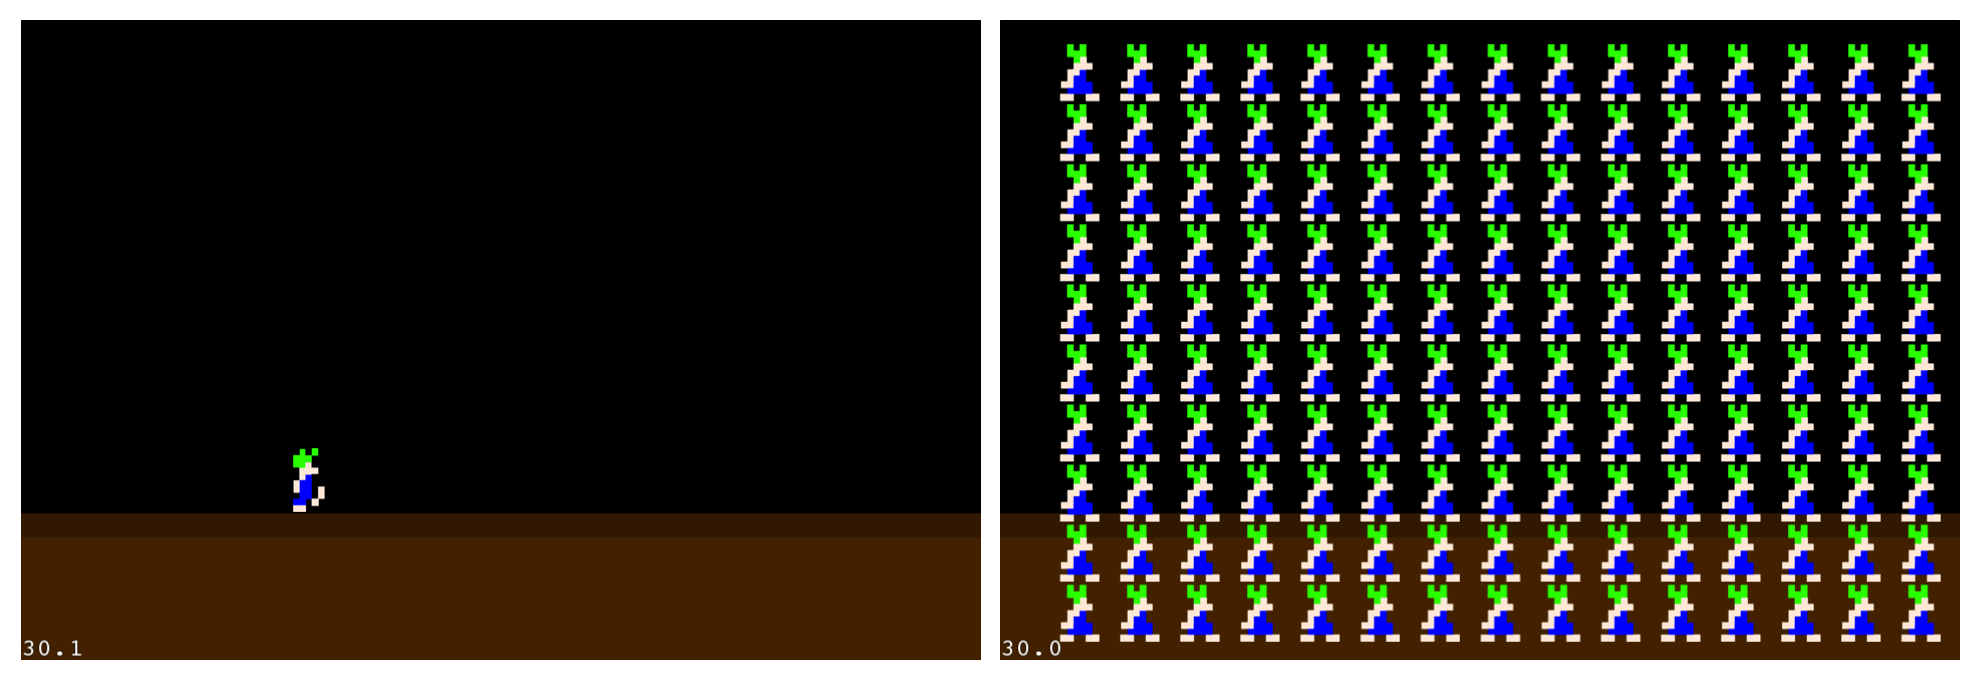
\includegraphics[width=140mm]{sources/images/InitialTests}
    \caption{Screens from my performance tests, both running at 30fps.}
\end{figure}

I carried out a few basic performance tests to see if there were any performance bottlenecks similar to the issues I had with JME. My first test was to add a single character to the scene, and animate it. My second test was to add more animating characters to see if there were any framerate issues; after adding 150 sprites, I was still achieving an impressive 30fps (see Figure 4 for screens). 

\section{Asset Production}

I also needed to create a variety of assets for my game (backgrounds, character sprites, menu items, fonts etc). The Cocos2D engine supports a variety of image file formats, including the lossless PNG format. For the creation of my graphical assets, I used an image manipulation program called \emph{Pixelmator} which exports to PNG as well as a number of other formats. I also needed to create texture atlases (or sprite sheets) in order to take advantage of Cocos2D's optimised sprite batch node feature (discussed more in the implementation section). For the fonts, I used a program called \emph{bmGlyph}, which is specifically developed for use with game engines that support the FNT file format.

\section{Version Control}

Using some form of version control system is a necessity in modern software development; it provides an easy way for multiple developers to collaborate on a single project (or even a single file) without causing file corruption. It is an invaluable tool for modern software development teams where it is not uncommon for developers to be in different cities or even continents. It also tracks all changes made throughout the development of the project. This is perhaps the most useful function of any version control systems as it not only allows the developers to see exactly what was changed (and by whom) in a project's history, but also means that were a mistake made, the project could easily reverted to an earlier state. Although I'm unlikely to experience any problems with file corruption as I'm the only one who will be contributing to the code-base, using a version control system still provides an incredibly useful way for me to not only track the progress of my project, but also as a way to incrementally back-up my project to ensure that any data loss is recoverable.

There are a variety of different source control systems available, such as CVS Subversion, Mercurial and Git. I decided to use Git as the version control system for my project as it is widely supported by many IDEs and other version control management software. I also generally prefer Distributed Version Control Systems (DVCS) as opposed to centralised systems for the reason that I like the freedom DCVS systems give you in terms of being able to work on a project without the need for an internet connection. DVCS systems also provide more security as each user has a backup of the entire system. However, this is not necessarily a benefit, as it could take up an inordinate amount of storage space were I working with many binary files (for example Adobe Flash files). In this case, using a DVCS would be unsuitable. The Git version control system is actually very simple; it tracks all files in a project, and each change made to the system (called a 'commits'). Specific commits can be 'tagged' to mark their significance; a feature which is normally used to mark releases of a project. I will be using a Git server hosted by GitHub to store the source code and documentation for my project. 

\section{Project Management}

To manage the progress of my project, I used a web-based application called ProjectPier which I installed on my web server so could be accessed from anywhere. Using this system, I split my project into a number of 'task-lists' for each component in my project's development; for example: asset production, game development, AI development, testing, etc. I also added milestones to my project to mark specific targets that I wanted to achieve by certain dates. Using this system, I could add individual tasks that needed to be completed, deadlines (or 'milestones') to mark specific targets in the development of my project. I could also use the system to create a wiki for my project containing useful information. 



%
% New part
%

\part{Planning}{This section covers the process of designing my system, from the initial concept art and art direction, to the system functionality modelling.}

\chapter{Artwork}
	
The first task I carried out when designing my game was to create some initial artwork. Not only would this help to define the look and feel of the game, but it would also help me to visualise how the levels could be structured, which would give me more of an idea as to exactly what kind of functionality was feasible. In addition to logos and some initial art direction, I also created the initial art for the agents, some sample screen artwork and some level designs.
	
\section{Logo Design}
	
I went through a few different iterations (see Figure 5), settling on a blue/white/black colour scheme. I wanted the art style to be clean and unobtrusive, so didn't want to use a lot of bright colours. I went for a mainly monochromatic colour scheme, with the blue used sparingly for emphasis. This would be the colour scheme that I would use throughout my game.
	
\begin{figure}[h!]
  \centering
    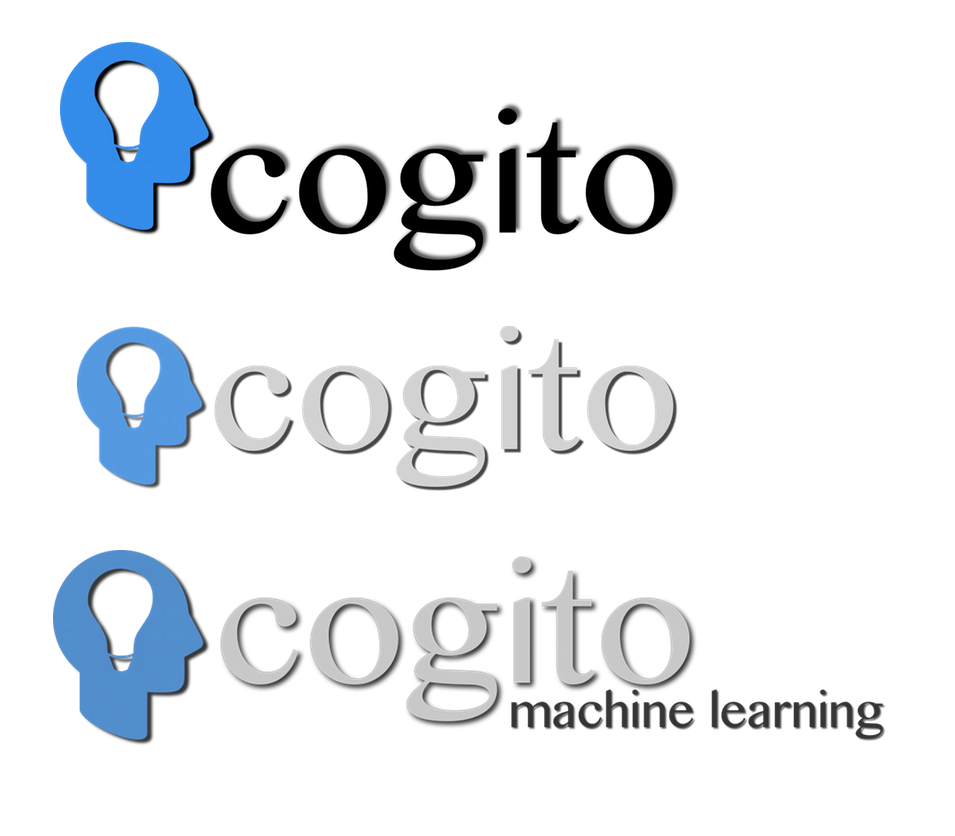
\includegraphics[width=90mm]{sources/images/cogito_logo1}
    \caption{Iterations of My Logo Design}
\end{figure}

\section{Game Design}

After settling on a colour scheme and basic art style, I then went about creating some mockups of various screens that I would be using in my game.
	
\begin{figure}[h!]
  \centering
    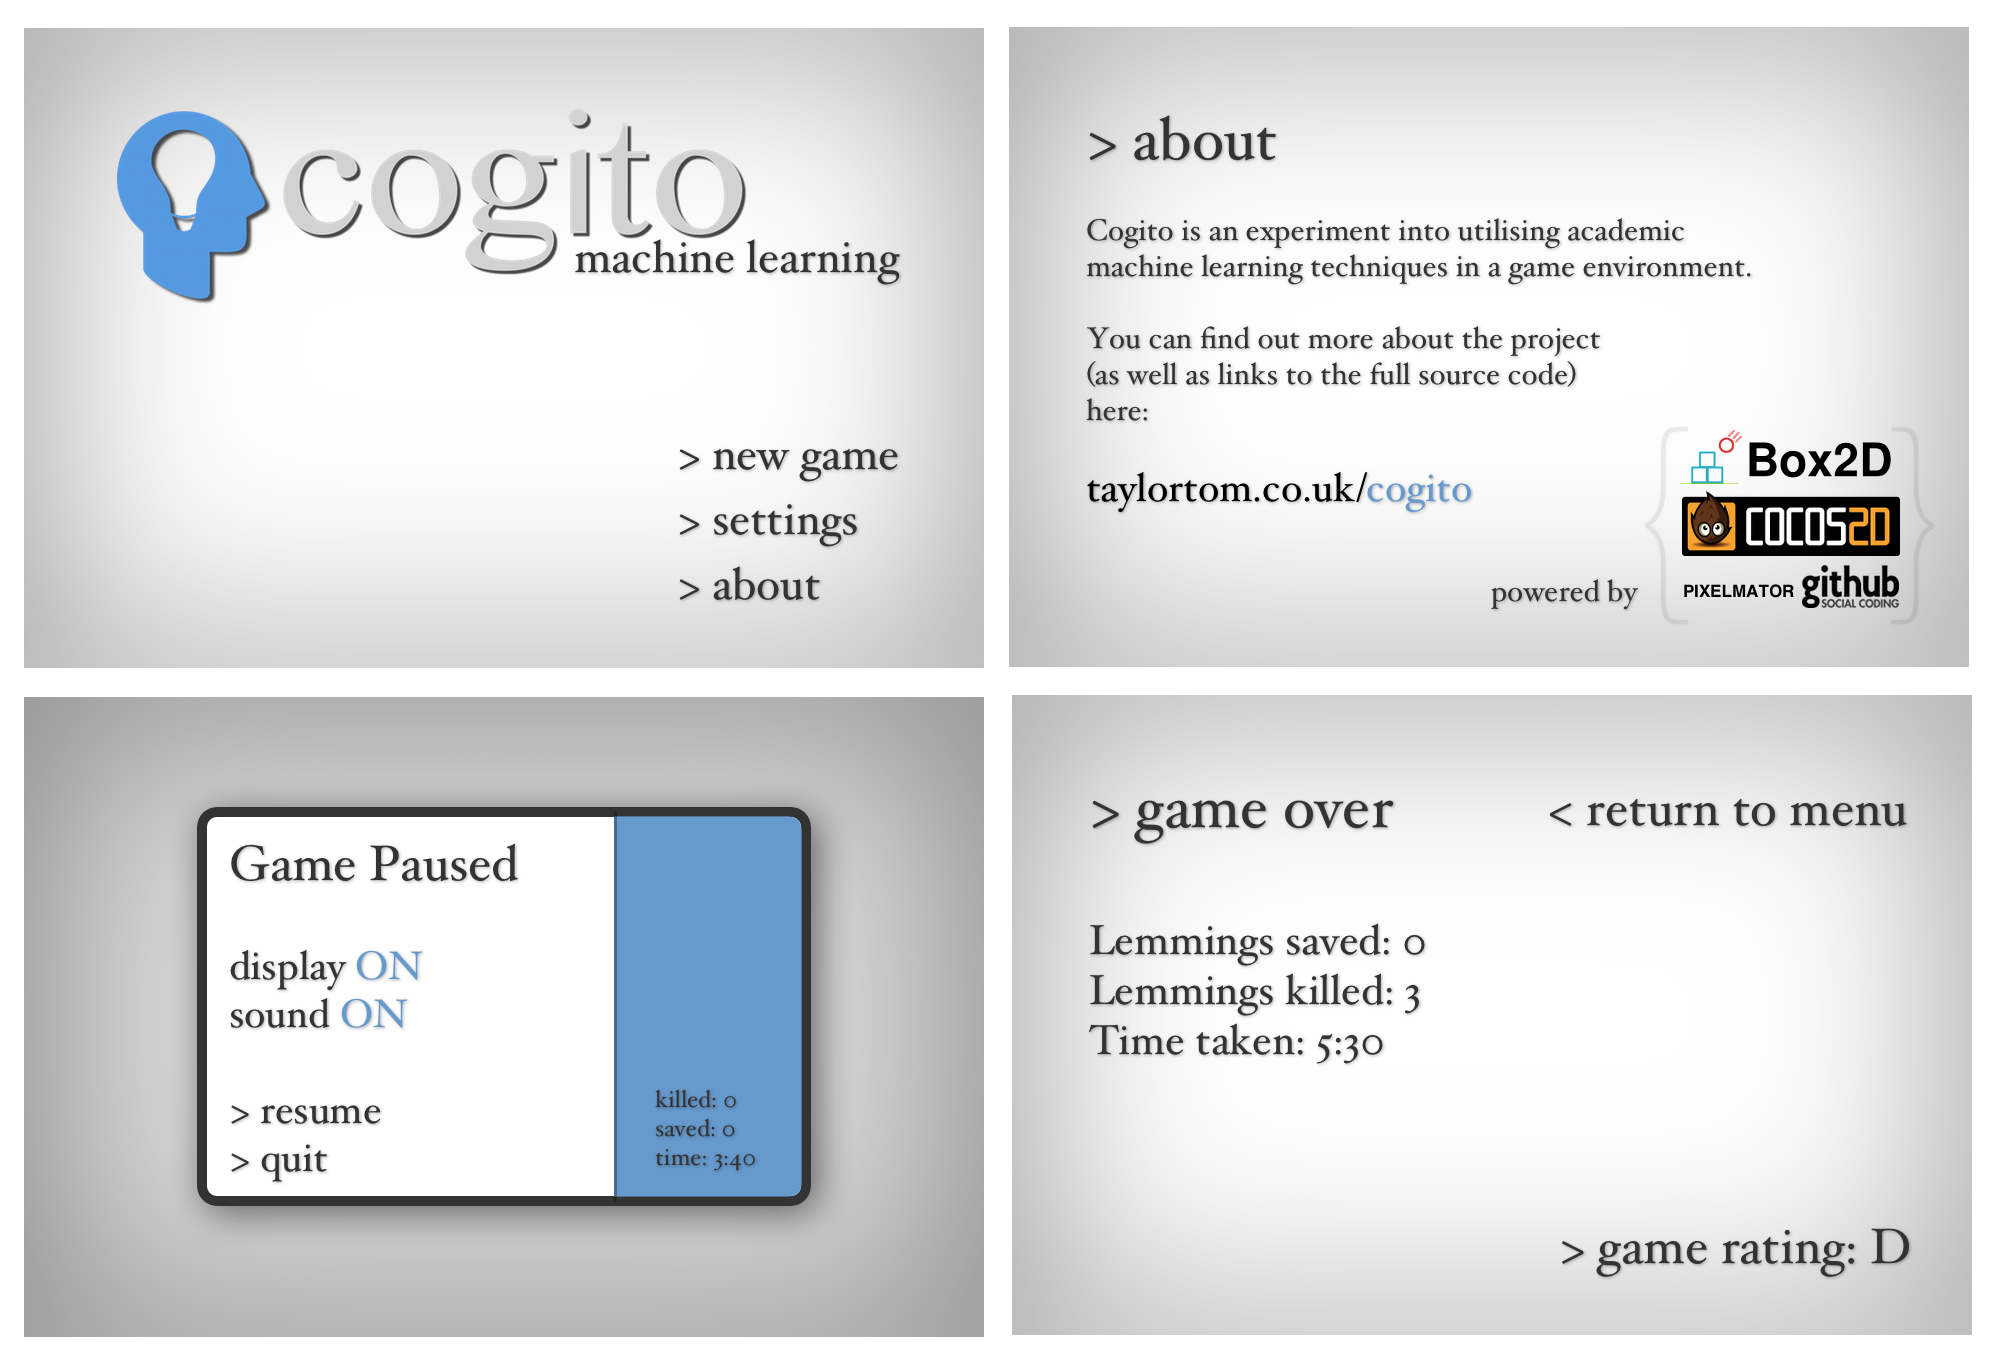
\includegraphics[width=140mm]{sources/images/Screens}
    \caption{Initial Screen Mockups and Art Direction}
\end{figure}

I also created a basic level design to give me more of an idea as to how a level might look. The idea of this was to get more of an idea of exactly how I might implement the level later; how the agents might transition between the different levels etc. I also decided to split the level into a number of `nodes' (visible in Figure 7). This would serve to simplify the agent's navigation, and is a similar idea to navigation meshes used in many games.  

\begin{figure}[h!]
  \centering
    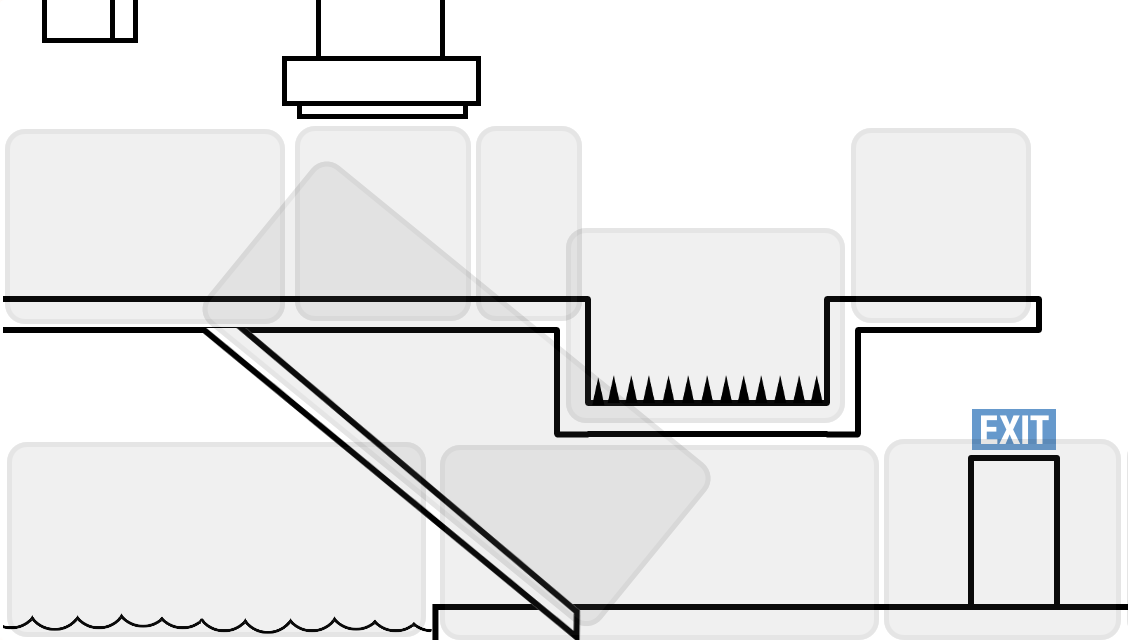
\includegraphics[width=120mm]{sources/images/LevelDesign}
    \caption{Initial Level Design}
\end{figure}
	
\section{Sprite Design}
		
I took a lot of guidance from the original sprite style and animation used in the original Lemmings game (see Figure 8). I decided to stay with the simple 8-bit art style for the sake of simplicity.
	
\begin{figure}[h!]
  \centering
    
\includegraphics[width=80mm]{sources/images/lemmings-walker-sprites}
    \caption{The Original Walking Animation Used in Lemmings}
\end{figure}
		
Using the above as inspiration, I created the walking animation frames, as well as the other animations required in my game (walking with helmet, open/use umbrella, floating, death). I used my chosen colour scheme for the agents to fit in with the rest of the art style.
		
\begin{figure}[h!]
  \centering
    
\includegraphics[width=60mm]{sources/images/Final}
    \caption{Final designs for agent sprites}
\end{figure}

I later added a faint outline to the agents, as I found when testing the game that the they became indistinguishable against the white background.
	
\begin{figure}[h!]
  \centering
    
\includegraphics[width=60mm]{sources/images/Lemming_walk_anim}
    \caption{The Final Walking Animation}
\end{figure}
	
\chapter{System Design}

After creating the initial artwork, I had to create a more concrete outline of the intended functionality for my game. From this specification, I could then start to design my system, structuring in into logical interrelated classes. To create a basic specification of my game, I split it into 3 logic components: the menu structure, the game component, and the AI system. I outline each briefly in this section.

\section{Menu}

Rather than just simply have the game start as soon as it is loaded up, I wanted to implement a simple menu system. This would also allow me to add other screens such as instructions for the player. I wanted the main functionality of the menu system to be as follows:

\begin{itemize}
	\item Have a link to the new game screen
	\item Have a link to game instructions
	\item Have a link to an `about' screen
	\item Be uncluttered
	\item Only to have one `level' (i.e. no complex nested menus)
\end{itemize}

Included in the menu component were two screens: the instructions screen, and the `about' screen. The former giving the player some basic instructions as to how to `play' the game, and the latter providing a bit of background information about the project.

\section{Game}

The `game' component encompasses the core functionality of the game (without the AI capabilities) such as displaying the graphics, controlling animations etc. My game component need to encompass the following:

\begin{itemize}
	\item Load and transition between the different scenes (i.e. menu \& game over scene etc.)
	\item Load game assets and external level file
	\item Animate game assets
	\item Build levels from the external assets
	\item Control the running of the game (game timer, pausing/resuming and exiting)
	\item Manage characters (adding, removing, watch for the end of the game)
	\item Display a game over screen with game rating
\end{itemize}

\subsection{Lemming Functionality}

In addition to the basic game functionality outlined above, I also needed to specify how I wanted my lemming game characters to function. 

\begin{itemize}
	\item Be able to move around the level
	\item Be able to change state as necessary
	\item Have basic collision detection
	\item Be able to animate
	\item Be able to detect if an end condition's reached
\end{itemize}

\section{AI System}

Rather than just simply have the game start as soon as it is loaded up, I wanted to implement a simple menu system. This would also allow me to add other screens such as instructions for the player. I wanted the main functionality of the menu system to be as follows:

\begin{itemize}
	\item Detect when agent has reached a decision point
	\item Be able to generate a list of possible actions (and choose randomly)
	\item Be able to dynamically create and maintain a knowledgebase of routes using the following learning types:
	\begin{itemize}
		\item Shortest route
		\item Decision tree
		\item Reinforcement learning (Q-learning)
	\end{itemize}
	\item Be able to use this knowledgebase to generate an optimum route
\end{itemize}

\section{Class Diagrams}

I created some initial class diagrams to specify how I intended to design the system. These classes show their intended functionality, and how they relate to other classes in the system. 

\subsection{Layers}

The layers contain the actual game content, such as background sprites, the character sprites, menu items, text labels etc. These are the initial specifications for the layers in my game (Figure 11).

\begin{figure}[h!]
  \centering
    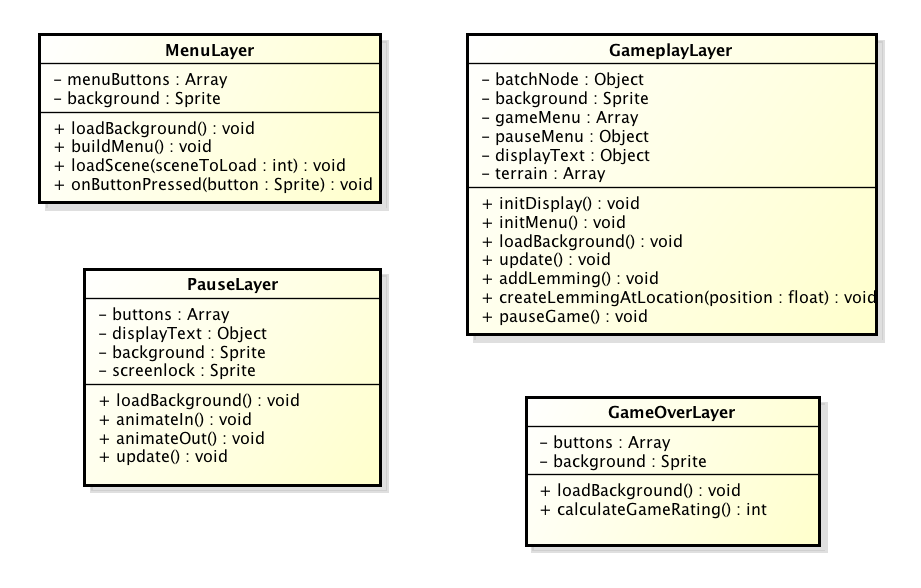
\includegraphics[width=130mm]{sources/images/Layers}
    \caption{The `Layers'}
\end{figure}

\subsection{Singletons}

I intended to use a number of classes using the singleton design pattern to manage the shared data in my game. I initially decided to use LemmingManager and GameManager singletons, although I ended up adding more in my final system (Figure 12).

\begin{figure}[h!]
  \centering
    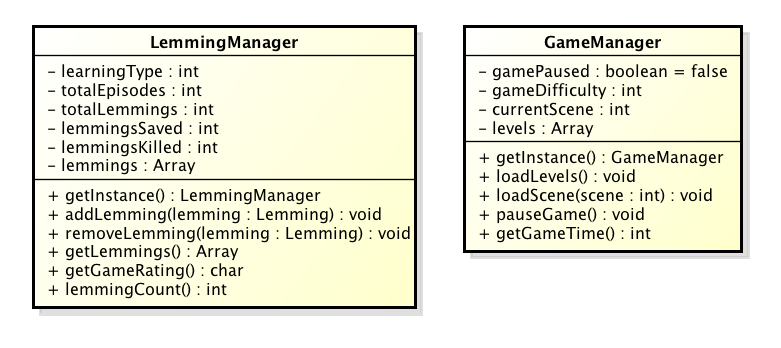
\includegraphics[width=110mm]{sources/images/Singletons}
    \caption{The Singletons}
\end{figure}

\subsection{GameObjects}

I planned to create a base class called `GameObject' which would be inherited by all of the game objects I would be using in my game. Objects such as the agents and the level terrain (Figure 13).

\begin{figure}[h!]
  \centering
    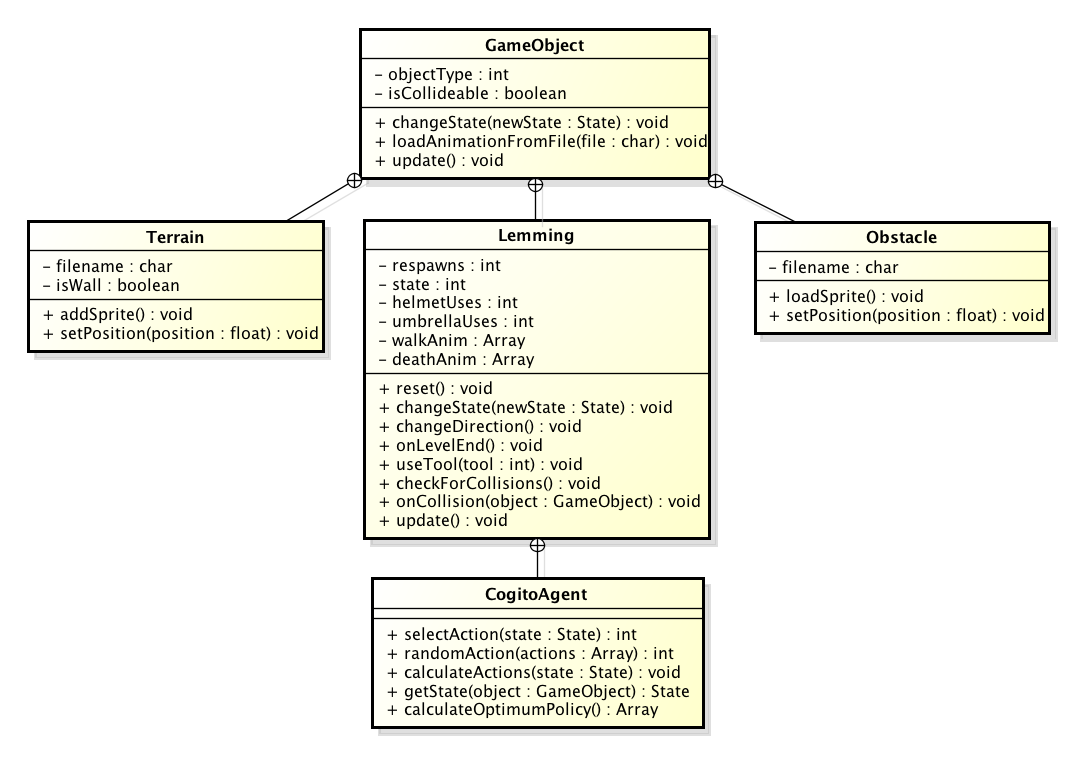
\includegraphics[width=140mm]{sources/images/GameObjects}
    \caption{The Game Objects}
\end{figure}
	
\section{Agent States}

I also created a basic state diagram to map out the intended states for my game characters (Figure 14).

\begin{figure}[h!]
  \centering
    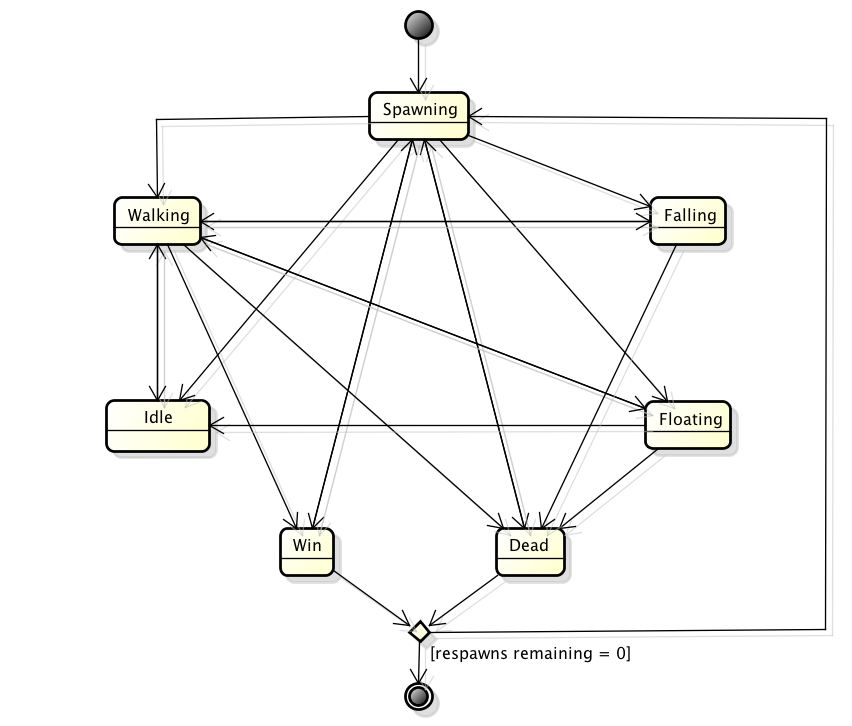
\includegraphics[width=100mm]{sources/images/LemmingStatemachine}
    \caption{Character States}
\end{figure}
	
	
\chapter{Social, Legal, Ethical and Professional Issues}

When designing my game, I had to consider a number of social, legal, ethical and professional issues to ensure that my product and its development complied to any applicable laws and ethical standards.

\section{Intellectual Property}

All of the intellectual property used in my game is my own, with the exception of the Cocos2D framework which I used. I have cited that I have used the engine in the game itself on the `about' screen. I have also included a copy of the relevant license in the source code. The engine is published under the MIT licence, which states that it is free to use in proprietary software provided that all copies of the software also include a copy of the license. A big benefit of the MIT license is that software which uses MIT-licensed code has no obligation itself to be published using the same license, and can be completely closed-source.

\section{Copyright Law}

In order to ensure that my product complied with copyright laws, I decided to create all assets needed myself. This ensured that I didn't need permission from any third parties prior to developing/releasing my product. All of the assets such as the backgrounds, logos and animations have been created by me solely for the purpose of this project.

\section{The Data Protection Act}

I don't store any personal data about the user in my game, so there are no issues regarding the Data Protection Act. The only information I collect is data regarding the agent's learning in the game, which is not transmitted to any source, but is simply used within the game to provide some basic stats about the system.

\section{Ethical Issues}

As I carried out my usability tests with the help of human subjects, I made sure that the subjects were kept completely anonymous and all information with regards to them confidential. There was no need for my to store any personal data about them, so this didn't present an issue.



%
% New part
%

\part{The Product}{This section gives a detailed description of the actual product, along with screens.}

\section{Introduction}



\section{Navigating}

Upon loading the game, you are greeted with the main menu screen. From here you can navigate to a number of other screens: start a new game, view game instructions, game stats and an `about' screen displaying some other useful information about the game.

\begin{figure}[h!]
  \centering
    
\includegraphics[width=70mm]{sources/images/Menu}
    \caption{Main Menu}
\end{figure}

\begin{figure}[h!]
  \centering
    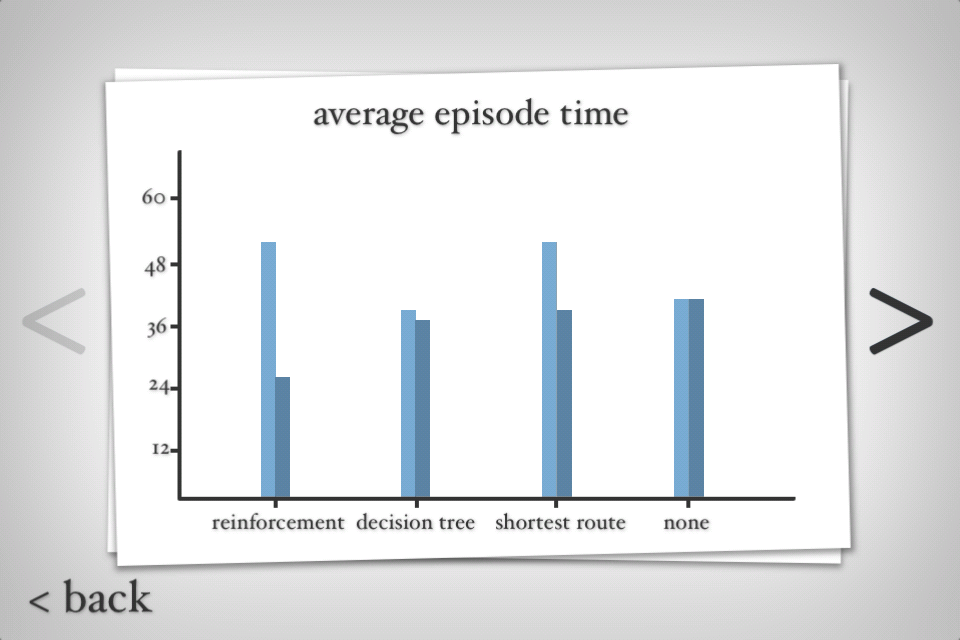
\includegraphics[width=70mm]{sources/images/Stats}
    \caption{Game Stats}
\end{figure}

\begin{figure}[h!]
  \centering
    
\includegraphics[width=70mm]{sources/images/Instructions}
    \caption{Instructions}
\end{figure}

\begin{figure}[h!]
  \centering
    
\includegraphics[width=70mm]{sources/images/About}
    \caption{About}
\end{figure}

\section{Starting A Game}

\begin{figure}[h!]
  \centering
    
\includegraphics[width=70mm]{sources/images/NewGame}
    \caption{New Game}
\end{figure}

\section{Playing The Game}

\begin{figure}[h!]
  \centering
    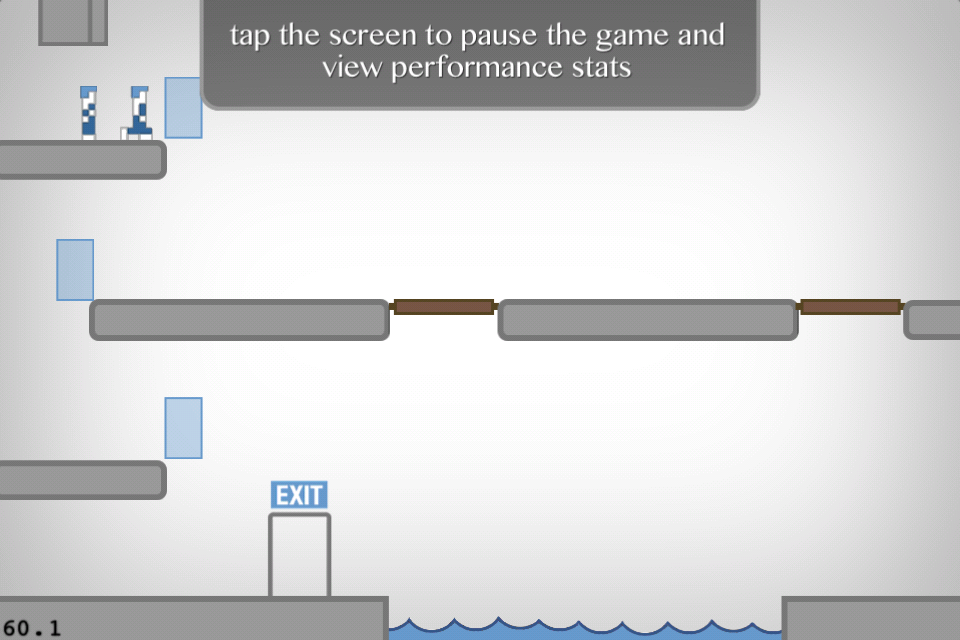
\includegraphics[width=70mm]{sources/images/DebugMode}
    \caption{Game Screen}
\end{figure}

\begin{figure}[h!]
  \centering
    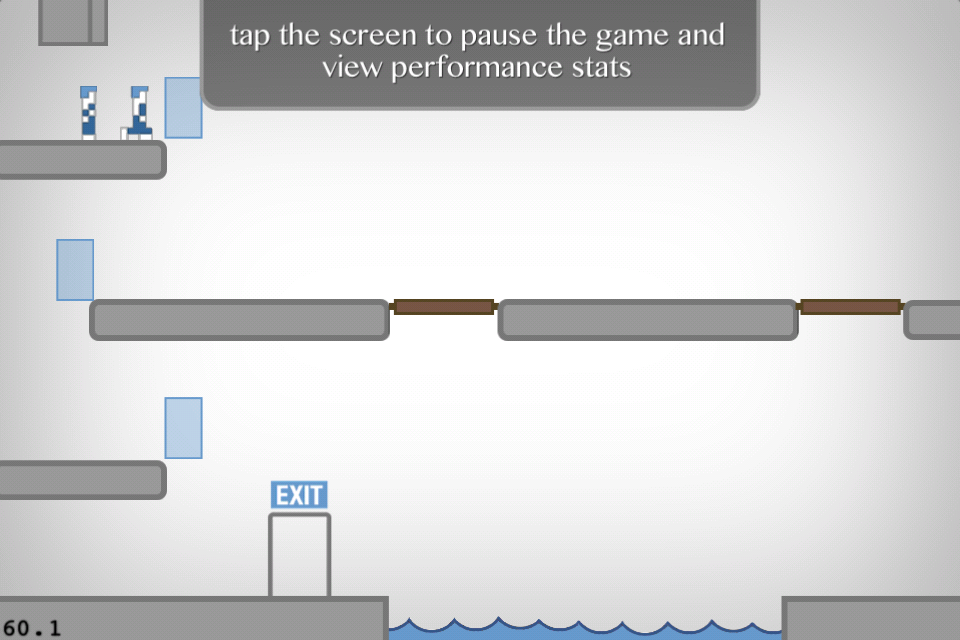
\includegraphics[width=70mm]{sources/images/DebugMode}
    \caption{Debug Mode}
\end{figure}


%
% New part
%

\part{Implementation}{This section covers the process of actually implementing my system, problems that I was faced with, and how I solved them.}

\chapter{Coding Practices and Structure}

When writing the code for my project, I tried to stick to standard code formatting conventions and use standard design patterns where possible, as outlined in this section.

\subsection{Code Structure}

When setting up all of my files, I followed a common layout/structure as standard good programming practice, to ensure that my code was as easily readible to others as possible. I tried to keep the formatting the same in all places, and used a clear informative commenting style.

\subsubsection{Commenting}

I made sure that all of my source code files follow a certain comment format. The filename, project name, class description and the date the class was created at the very top of the file. Each method is then commented, with a brief description and any parameters/return variables specified. I tried to avoid commenting variables wherever possible, instead choosing to use variable names which are self-descriptive. See below for comment formatting.

\begin{lstlisting}
//
//  File name
//  Project name
//
//  Class description
//
//  DD/MM/YYYY: Created class
//

/**
 * Method description
 * @param any parameters
 * @return the returned objects
 */\end{lstlisting}

\subsubsection{Methods}

The format of my method headers is fairly standard, however, I prefix all method parameters with an underscore as it helps to clarify which variables in a method are parameters if quickly scanning the code.

\begin{lstlisting}
-(void)addLemming:(CCSprite*)_lemmingToAdd;
\end{lstlisting}


\subsection{Singleton Classes} 

I made a lot of use of the singleton design pattern throughout my project to create various 'manager' classes to deal with the shared data in my system. A singleton class is a special kind of class which only has one instance; calling a singleton instance will always return the one instance of the class, regardless of which class called it. The major benefit of using the singleton pattern being that you only need to store the data in one location, which can then be accessed by any class anywhere in the program (provided that the access to the data is restricted to a single thread at a time to avoid concurrency issues). My LemmingManager class which handles all of the agents in the game is an example of where I have used this pattern. It hold the only list of the characters in the game, and contains the functionality to add and remove lemmings among other things.

\subsection{Constants} 

I created a file to contain the read-only constant variables used in my program (for example the framerate, the default font filename and the various rewards associated with reinforcement learning). Moving all of these variables into a single separate file means that Each constant in this file follows the standard naming convention for constants (i.e. starting with a "k"). This is a legacy feature from the pre-Mac OS X days, possibly back when the Mac OS was written mostly in Pascal. 

\subsection{Datatypes} 

In addition to the constants file, I also created a similar file which contained many common datatypes which I would be using in my game. Types such as machine learning type, terrain type, character state, game rating and so on. As with the constants, this meant that I could keep all of the needed datatypes in a common location for easy access.

\subsection{Utility Methods} 

I created a Utils class with some useful static-access 'utility' methods which I was likely to want to use a lot in my game; functions such as random number generation, enumeration-to-string conversions, and timestamp generation. It made sense to create a separate class with all of these types of methods because it not only cut down on the amount of code that I had to write, but also meant that were I to find a bug in my random number generation code for example, I would only need to fix the bug in one place, rather than having to go and search every source file for occurrences of the broken code. 

\chapter{Game Component}
		
\section{Code Structure/Features}

Before I could build any learning into my project, I first had to create the underlying game component which would run it. As I was using the Cocos2D engine, a lot of the very low-level functionality had been taken care of. For example, the direct OpenGL ES calls needed for loading and binding textures were all contained within the CCSprite class. However, I still needed to take care of loading levels, adding objects, game characters, animating characters etc.

\subsection{Cocos2D} 

The Cocos2D framework comes with a very useful code library with various optimisations and utility methods which I made use of when implementing my game.

As previously mentioned, Cocos2D comes with a number of different base classes which can be used and take care of a lot of the very low-level OpenGL API calls. These classes have a heirarchical structure, using an analogy of film production to make this easy to understand. At the highest level is the CCDirector class which, as one would expect, controls the running of each individual level in the game (known as scenes). Scenes are essentially any new `screen' in the game, so are not necessarily just game levels, but can also me menu systems, game over screens and so on. Each scene consists of one or more layers which contain the actual game objects (for example background images, any level terrain and the game characters). The game objects (known as sprites) are at the bottom of the heirarchy and are just essentially an image with no real functionality by default.

The Cocos2D framework is loaded via the AppDelegate singleton class, which controls with the basic running of the iOS application; what should happen when launching the app, when the user closes the app, when the app is sent to the background etc.

In addition to the basic classes mentioned above, Cocos2D comes with a number of other useful features, such as the ability to add `transitions' in between scenes. The Cocos2D library also comes with a very useful CCAction class which allows the programmer to easily ass basic animations to sprite objects by simply specifying a start and end position and a duration. The class then creates an animation by interpolating between these two points. I use these actions in a number of places throughout my game, from animating the main menu items, switching graphs in the game stats screen, moving the agents in the game, and animating the game's pause menu. 

There are also some highly optimised data structures available, the most prominent being the CCArray class, which is a basic collection class which has been optimised for high-performance, with some methods that allow fast enumeration.

\subsection{Physics}

I initially intended to use one of the physics engines bundled with Cocos2D for the physics in my game. However, as the only physics required in my game was some basic collision detection and some way to simulate the agents `falling', I decided to write the required code myself to cut down on the processor time required. The other benefit to programming the physics and more specifically the collision detection myself is that I could customise which objects were included in the collision checks. This meant that I could optimise performance even further by ignoring any agent-to-agent collisions for example.

For the actual collision detection itself, I used basic bounding box detection as I had no need for anything more accurate. I made use of a method in the CCNode class (which my agents inherit from) which generates a bounding box for any given sprite. To detect whether any two objects were colliding, I made used of a utility method from the iOS code library \emph{CGRectIntersectsRect} which as the name suggests, checks if two rectangle objects intersect each other.

To simulate the agents `falling', I simply used a `CCAction' which basically creates an animation by interpolating between the start and end positions, similar to a `tween' in Adobe's ActionScript/Flash platform. 

\subsection{Levels} 

When it came to designing how the levels would work in my game, I wanted something which was very flexible, so that I could easily add extra levels (or modify existing ones) with a minimal amount of work. The way that I decided to do this was to create a number of generic assets which I could re-use in each level. Things such as platforms, water hazards, trapdoors etc. This meant that when I wanted to add an additional level to the game, I could simply specify the positioning of these existing elements, rather than having to create new level assets per level. By using re-usable assets, not only was adding new levels a lot simpler, it also meant that I could drastically cut down on the amount of disk-space that my game needed.

To accompany the assets, I also needed some way to specify the layout of each level, as well as other level specific data. To accomplish this, I used the natively supported Property List (plist) file format. Plist files are simply XML files of dictionary objects, consisting of a key object (usually a string), and a `value' object. One of the advantages to using the plist is that it's easily editable in any text editor. It also supports a variety of datatypes, such as strings, numbers (ints, floats, etc) and dates. Dictionaries can also be nested inside each other for even more flexibility. 

I use one plist file which specifies the levels in my game, along with certain level-specific information such as difficulty, number of tool uses etc. This file is loaded in, which tells the system how many levels need to be loaded, as well as their names. I then created a plist file for each level, which stored the positions of each piece of terrain, the type of terrain, and in some cases whether the terrain was collideable (this was enabled by default, so was only included if the object was to be removed from collision detection).

After loading in these plist files, I needed to translate the loaded data to into tangible game objects which could then be added to the game. To do this, I created terrain (i.e. platforms and floors) and obstacle (i.e. water, stampers etc.) classes which would encapsulate the required functionality. These classes contained the code necessary to create the sprites from the correct image files, and store the coordinates of the sprites according to the data loaded from the level's plist file. I also created a TerrainLayer class too keep all of the terrain objects separate from the other game objects. This class also deals with the actual loading of the plist files

Initially, I planned to have levels of varying difficulty, with an option on the new game screen to allow the user to select a difficulty. However, I found it difficult to determine what an 'easy' level should be for example, and so the final game just assumes all of the levels are the same difficulty. 

\subsection{Basic Agent Functionality}

Before I could program any of the machine learning into my agents, I first needed to set up some basic functionality such as animating and moving the agents and the ability to change state as well as some other basic behaviour.

I first programmed the animation for the characters, which involved splitting the animations into individual frames (see Figure 6) which could then be loaded into my game. To specify the frames needed for each animation, I created an external plist file which also listed the order of the frames, and the animation's length. 

\begin{figure}[h!]
  \centering
    
\includegraphics[width=60mm]{sources/images/Lemming_walk_anim}
    \caption{Frames Used for the Agent's Walking Animation}
\end{figure}

In addition to the animations, I also needed to set up some other basic behvaiour. I used a finite state machine which encapsulated all of the basic states for my agents: spawning, falling, idle, walking, floating, dead and win (i.e. reached the exit). Using this state machine, I could adjust the behaviour of the agents according to various in-game stimuli, and play any animations as appropriate. An example being when a falling agent collides with the ground, it transitions to the walking state. I also had to code a basic `fall timer', which counted how long an agent had fallen for, setting the next state to either walking, or dead if the fall was longer than a certain threshold. By this stage, I had set up my agents to spawn into the level at the correct point and move around the level from left to right, until they reach an immovable object at which point they turn around. I had added terrain objects and obstacles which changed the agent's state as appropriate (to `dead' if agent falls into water for example). The agents would respawn in killed, and the game would end if they successfully reached the level exit. At this point, my agents acted exactly as the characters in the original \emph{Lemmings} game, with no reasoning or other `intelligent' behaviour attached to them.

\subsection{Performance Optimisations} 

As already mentioned, Cocos2D offers a variety of performance optimisations specifically tailored for developing games. One such optimisation is the 'CCSpriteBatchNode'. It is not uncommon to experience poor performance when there are a large number of objects onscreen at once. 

For each sprite, OpenGL ES must first bind to the texture, and then render the sprite. As more and more sprites are added to the screen, it isn't difficult to see that the number of calls to OpenGL will steeply increase too, with every call costing a few CPU cycles. It is basic common sense to see that the game will run faster the fewer calls to OpenGL are made. 

The CCSpriteBatchNode is a Cocos2D class which has been created to help with this problem. The CCSpriteBatchNode works by taking a single texture which contains all of the textures needed by the current scene (called a texture atlas, see Figure 7), and sends all of the images for rendering to OpenGL at once, rather than individually. This essentially reduces the number of bind calls needed from O(n) to O(1) (in Big-O notation). Using texture atlases also cuts down on the amount of memory needed to store each individual image. In some version of the iOS, textures were required to be stored in sizes of the poet of two (64, 128, 512 etc.). This meant that the textures would often have a lot of unnecessary white space around the image, which obviously takes up extra memory; something which even with todays devices is not a commodity. An additional optimisation which can be made regarding the textures is to use the compressed PVR CCZ file format. In addition to saving disk space in terms of the actual size of the image, the PVR CCZ format is supported natively by the iPhone's GPU, and can be loaded directly onto the GPU without the need for conversion.

\begin{figure}[h!]
  \centering
    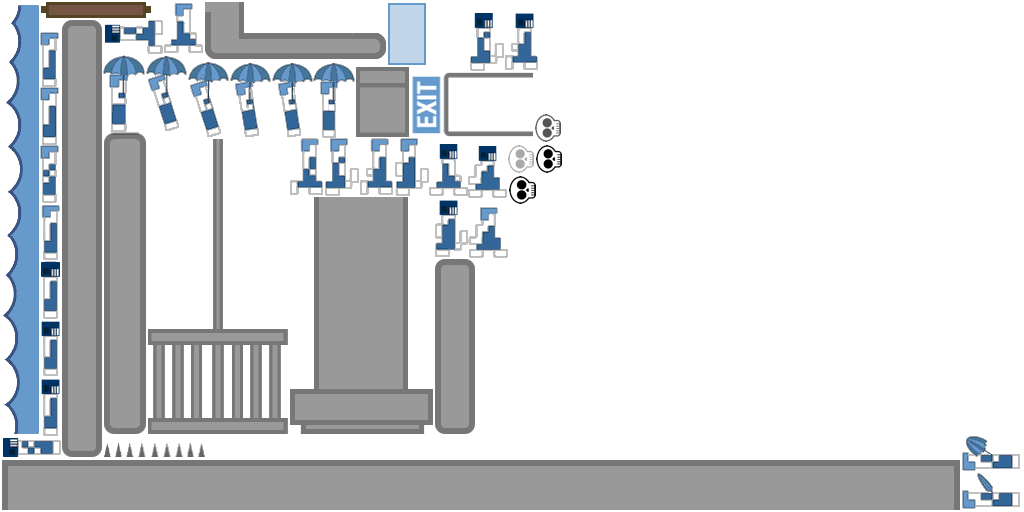
\includegraphics[width=100mm]{sources/images/Texture_atlas}
    \caption{An Example Texture Atlas}
\end{figure}

\subsubsection{Random number generation} 

Although it may not seem like a likely source for a performance bottleneck, the random number generator (RNG) I chose to use could have a noticeable impact on performance. Based on some very quick tests carried out by a poster on the official Cocos2D forums, I was surprised to see the difference in speed between different RNG (see Figure 8) \cite{:2011zt}. Typically, the RNG I had chosen to use (arc4Random) was by far the slowest method tested. Based on the tests carried out, I instead decided to use the CCRANDOM\_0\_1 function, which was shown to be 5 times quicker. Although the tests carried out on the forum were tested by performing 5 million iterations of the algorithm, far more than I would ever need to use, every performance enhancement helps.
	
\begin{figure}[h!]
  \centering	
	\begin{tabular}{|l|c|c|}
\hline
Algorithm & Device Time (secs) & Simulator Time (secs)\\ \hline
\multirow{5}{*}{Ranrot} & 0.037202 & 0.004751 \\
 & 0.036453 & 0.004786 \\
 & 0.037306 & 0.005023 \\
 & 0.036244 & 0.005536 \\ 
 & 0.037261 & 0.005243 \\ \hline
\multirow{5}{*}{UNI (multiply with carry)} & 0.287225 & 0.014551 \\
 & 0.286778 & 0.014798 \\
 & 0.285554 & 0.016061 \\
 & 0.286738 & 0.014633 \\
 & 0.288803 & 0.016177 \\ \hline
\multirow{5}{*}{CCRANDOM\_0\_1 (C random)} & 0.504273 &  \\
 & 0.498741 &  \\
 & 0.572036 &  \\
 & 0.498766 &  \\
 & 0.503112 &  \\ \hline
\multirow{5}{*}{xorrand} & 1.880982 & 0.093661 \\
 & 1.947728 & 0.101897 \\
 & 1.869296 & 0.090943 \\
 & 1.866257 & 0.091044 \\
 & 1.868058 & 0.096747 \\ \hline
\multirow{5}{*}{arc4random} & 2.970779 &  \\
 & 2.782961 &  \\
 & 2.973706 &  \\
 & 2.781113 &  \\
 & 2.785057 &  \\ \hline
\end{tabular}    \caption{Performance Tests of Random Number Generators}
\end{figure}

\subsection{SlideViewer}

As I had a number of screens which were intended to present information to the player, I wanted to design some kind of reusable asset which could be dropped into my game and used to display this information. To this end, I created the \emph{SlideViewer class}, which as the name suggests, consists of a number of `slides' (which are simply images), which can be navigated through at the player's leisure.

The viewer is an extension of the base Sprite class, and so can be added to any other layer or sprite, and is extendable to cope with any number of slides.
		
\section{Problems Faced} 

Something which I found particularly tricky about using Objective-C over a language like Java was the memory management. Learning Objective-C really emphasised to me how much the Java runtime shields the programmer from the low-level bugs associated with memory management thanks to its garbage collector. In Java, memory is reserved for an object simply by using the 'new' keyword, and memory is automatically released when that object goes out of scope and is no longer accessible. On the other hand, languages such as Objective-C  require manual memory management, meaning that every object created needs to be manually released by the programmer when finished. While the Objective-C language does come with a few optimisations which make memory management easier, it still caused me a number of problems. 

I found that the biggest problem with memory leaks is that they can often go undetected, only to cause the program to unexpectedly crash later on down the line. For this reason, they can be notoriously difficult to track down. I discovered a particularly nasty bug for example in my game's update method for example, which is called every frame, whereby I was allocating an array to hold all of the game objects, but failing to release the memory at the end of the method. This was a relatively small leak, but it was causing my game to drop 10+ frames per second if run for over 10 minutes.

I found another seemingly insignificant bug in my update method which was causing me to drop 15 frames per second after the game had been running for about 15 minutes. The bug was caused by a careless error I made when initialising the game. When the game was first initialised, I wanted to create a list of all collideable objects, for use in collision detection later. To do this, I put code in the update loop which added every object to a list. However, rather than just adding the objects once when the game was initialised, I found that I was re-adding each object every frame, causing a huge issue with performance. After just 10 seconds, I found that my list of collideable objects contained over 10,000 objects, which was obviously causing big problems when it came to my game trying to check for collisions.

Xcode comes with a very useful set of performance analysis tools called 'Instruments' which can be used to establish any memory-related or runtime issues, such as memory leaks etc. Instruments allows you to test your app in `profiling' mode, which tracks what memory has been allocated, and suggests areas where memory leaks may occur.

Carrying out this project really taught me the importance of keeping a close eye on what memory I was allocating and where it was being released. What may at first seem like a negligible memory leak can build up over time, and combined with other similarly small memory leaks, can cause big problems with your programs performance. I would even go so far as to say that these smaller memory leaks are even more troublesome than the bigger ones, as they are much harder to track down, and are often more widely spread, and therefore more difficult to fix.

Another problem I frequently came across which couldn't happen in memory-managed languages like Java was that of uninitialised variables. Whereas in Java, whenever you declare a new variable, it's automatically initialised with whatever the default value may be, you get no such privilege in Objective-C. When you declare a variable in Objective-C, it stays uninitialised until you specifically set it. This caused me the biggest problems with arrays; trying to access an uninitialised array wouldn't cause a compiler error, but would cause an unexpected crash at runtime.

\chapter{AI Component}

After the core game component had been implemented, I could start to build the AI learning system. My first task was to update the levels 

\section{Level Structure}

In order to simplify the decision making process, I split my levels into a number of `nodes' similar to the navigation meshes used in many games (See Figure 9). These nodes represent decision points in my levels; areas where there are more than one possible path forward, where the agent has to decide which route to take. As trapdoors had already been placed in the level, these were used as one type of decision node. I also needed to create an additional invisible decision object which could be at the end of platforms or anywhere where I couldn't place a trapdoor. 

\begin{figure}[h!]
  \centering
    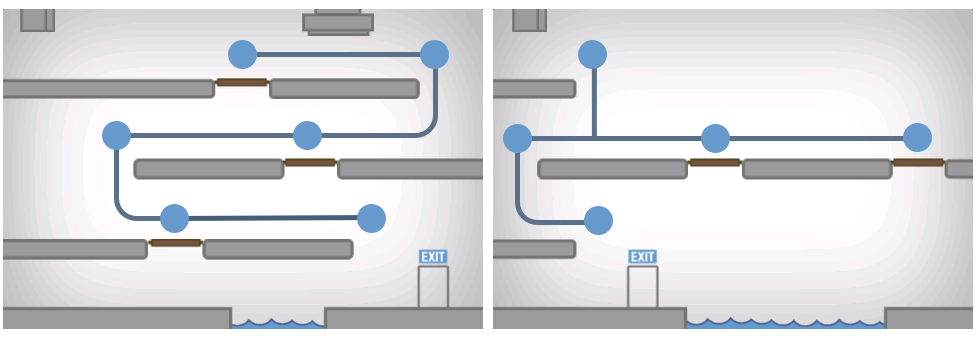
\includegraphics[width=140mm]{sources/images/LevelNodes}
    \caption{Decision Node Graphs for Two Levels}
\end{figure}

\section{Learning Agents}

In my final game, I implemented three alternative methods of learning: a shortest route method, a modified decision tree method, and a reinforcement learning method using the Q-learning algorithm. I explain the different implementations used in my game in this section.

As I intended to implement more than one learning technique, I designed the code for my game characters in such a way that the AI was completely self-contained in its own class. Not only is this generally good object-oriented design, but it also meant that to use a different type of learning, all I had to do was to link the relevant class, no other changes were required. This functionality could be neatly implemented in a switch statement (See figure 9)

\begin{figure}[h!]
\begin{lstlisting}
switch(learningType) 
{                
	case kLearningMixed:
    	// randomly choose a learning type
        learningType = [Utils generateRandomNumberFrom:0 to:kLearningMixed]; 
        break;
                
    case kLearningReinforcement:
        class = [QLearningAgent class];
        break;
                
    case kLearningTree:
        class = [DecisionTreeAgent class];
        break;
                
    case kLearningShortestRoute:
        class = [ShortestRouteAgent class];
        break;
         
    case kLearningNone:
        class = [CogitoAgent class];
        break;
                
    default:
        break;
}
\end{lstlisting}
\caption{Switch Statement for Setting Learning Type}
\end{figure}

As outlined in my initial design, the learning agents begin the game in a `learning mode', in which they have a set number of lives or `episodes'; the number of learning episodes is set by the player before the game begins. During learning mode, the agents navigate the level and choose actions at random, building up their knowledgebase. 

I initially planned to set up the learning such that after the first episode, the agent would cease to act randomly and apply its knowledge. However, I found that doing this made it extremely difficult to measure the improvement in the characters, as once they reached the exit, the game was over. Instead, I decided to implement the learning mode which avoids this issue. Additionally, by programming the agents to act randomly throughout the learning mode meant that more optimal routes were found in less time, due to the fact that there was no `exploitation' of current knowledge at this stage. In many reinforcement learning systems, the system begins to exploit the learnt knowledge much earlier on, which brings with it the added issue of balancing the exloitation of existing knowledge with the exploration of new terrain. 

After all of the learning episodes have been completed, learning mode ends the agent then applies the knowledge it has learnt to attempt to reach the exit safely.

\subsection{Cogito Agents}

I created a base class called \emph{CogitoAgent} to contain the common functionality which would be shared between all types of learning. Its most basic function is to detect when an agent has reached a decision node, at which point it chooses a random action from those avalable. The basic decision process is as follows:

\begin{enumerate}
	\item Agent collides with decision node
	\item Agent gets the current state
	\item Action chosen based on the current state
	\item Takes action
\end{enumerate}

The class also keeps track of the number of learning episodes used by the agent, and ends the learning mode when all episodes have been completed.

\subsection{Shortest Route Agents}

The Shortest Route agent is the simplest and most naive of all of the learning types. Shortest Route agents record the routes which have been taken during the learning mode. I created a Route class to simplify this, which itself consists of an array of `nodes' and a boolean flag which stores whether or not the route was successful (i.e. if the agent survived or not). Upon completion of the learning mode, the Shortest Route agent checks all of the routes taken, chooses the shortest one, and takes it. If there happens to be several shortest routes of the same length, the agent doesn't attempt to compare the routes, but just picks the first one it finds. If the agent failed to reach the exit during the learning mode, it simply acts randomly.

\subsection{Decision Tree Agents}

As shown in my research, decision tree learning is usually used for classification problems, whereby an agent finds itself in a certain situation, and it uses a decision tree to try to `classify' the situation using knowledge it has gained from experience. Initially, I planned to use this approach in my game. However, I felt that it was an overly complex solution to what is a relatively simple game concept. I didn't think that there was any point in trying to create diverse obstacles which required the agent to have to classify them; it just seemed unrealistic. I felt that trying to use classification techniques to solve my problem of terrain navigation was inappropriate
 
Instead, I decided to use tree structures to allow my Decision Tree agents to function in a similar way to the Shortest Route Agents. Like the Shortest Route agents, the Decision Tree agents record the routes taken, with the shortest routes being chosen after the learning mode is complete. However, there are some subtle changes which make this method more accurate than the Shortest Route method. The obvious difference is that the routes are stored in a tree structure, which is built dynamically as the agent experiences the world. 

To implement the tree structure, I created a \emph{TreeState} class. The class stores references to the parent and child nodes, and has code to add child nodes to the tree. There is also a boolean flag which stores whether the particular TreeState is a leaf node.

To calculate the shortest route, I need to search the tree. I do so by checking every node using a simple depth-first search. When a leaf node is found (and the node is an exit), I recursively move back up the tree to store the route. While this kind of search is very poor speed-wise, it ensures the tree is methodically searched. Were I traversing a much larger tree such that performance became an issue, I could a heuristic search method such as A* to provide an approximate solution. As it happens, my levels are small enough to make my brute-force search a feasible solution.

When searching for the optimum route, the routes are all given `weightings'. The weighting for a route is based on the number of tools used in that route; a route with no tool uses has a weighting of 0, with the weighting being incremented by 1 for every tool used.

\subsection{Reinforcement Agents}

The final and main type of learning which I implemented in my game was reinforcement learning. Based on my research, I decided that the Q-learning algorithm was the most appropriate for solving my problem.

I needed to decide upon what values to use for the rewards in my system. Although reinforcement learning systems tend to use values less than 1.0, I instead decided to use rewards of less than 100, just to make the values more manageable and avoid a lot of decimal places (see Figure 11 for values).

\begin{figure}[h!]
\centering
\begin{tabular}{| l | c |}
  \hline
  State  & Reward Value \\
  \hline
  Reached Exit    &  100.0 \\
  Died   		  &  -100.0 \\
  Used Tool       &  -7.0 \\
  Other  		  &  -2.0 \\
  \hline
\end{tabular}
\caption{Table of Reward Values}
\end{figure}

I used the same values for the win/death rewards (albeit one +100 and one -100) so that both states were regarded equally `important' by my learning agents. In addition to these rewards, I also added a small negative reward for any tool uses by the agent (i.e. umbrella/helmet uses). This ensured that the agent resisted using a tool wherever possible; tools are a finite resource, and so should only be used where no `cheaper' alternative exists. Using this small negative reward ensures that the agent will always choose the standard basic actions (i.e. left, right, down) over using a tool. While conducting my research, I came across a lecture on reinforcement learning given by researcher Andrew Ng in which he proposes associating a small negative with all moves \cite{Ng:uq}. I decided to do this in my own game, as it encourages the agents to use the shortest route possible by adding a greater penalty to longer routes. The reward values are stored in my \emph{Constants file}.

After setting up the rewards, I then needed to implement the actual learning. The basic operation of the reinforcement learning is as follows:

\begin{enumerate}
	\item Agent collides with decision node
	\item Agent gets the current state
	\item Q-values for previous state/action are updated according to outcome
	\item Action chosen based on the current state
	\item Takes action and updates state
\end{enumerate}

In my implementation, I chose to update the Q-values asynchronously (i.e. updating individual Q-values at each decision made), rather that to update all Q-values at set intervals (synchronously). I chose to update my Q-values asynchronously simply because I felt it was logical to do so, and was slightly simpler to implement. Both methods are acceptable to use with Q-learing, and have no major impact on the outcome of the algorithm.

To calculate the new Q-values according to the algorithm described in my research:

\begin{equation*}
	Q(s_t,a_t) \Leftarrow Q(s_t, a_t) + (1 -\alpha_t) + \alpha[R(s_t) + \gamma max Q(s_{t+1}, a_{t+1})]
\end{equation*}

To make my code more readable, I split the algorithm into logical parts and stored these parts in variables. For example, I created a variable for the old Q-value (i.e. $Q(s_t, a_t)$) and a variable with the maximum expected Q-value (i.e. $max Q(s_{t+1}, a_{t+1})$). My implementation of the algorithm is included in Figure 12.

\begin{figure}[h!]
\begin{lstlisting}
/**
 * Updates the Q-values
 * @param the state to update
 */
-(void)updateQValues:(QState*)_newState
{    
    if(currentState == nil) return;
            
    float oldQValue = [currentState getQValueForAction:currentAction];
    float maximumQValue = [_newState calculateMaxQValue];
    float reward = [_newState getReward];
    
    // apply a negative reward if using a tool
    if(reward == kQDefaultReward) 
    {
        switch (currentAction)
        {
            case kActionDownUmbrella:
            case kActionEquipUmbrella:
            case kActionLeftHelmet:
            case kActionRightHelmet:
                reward = kQToolReward;
                break;
                
            default:
                break;
        } 
    }
        
    float updatedQValue = oldQValue * (1 - kQLearningRate) + kQLearningRate 
    	* (reward + kQDiscountFactor * maximumQValue);
    [currentState setQValue:updatedQValue forAction:currentAction];
}
\end{lstlisting}
\caption{Method to Update Q-values}
\end{figure}

The learning rate which I use in my algorithm is largely down to trial and error, and is set at the value that I felt worked best in my game. My research was very helpful in guiding the values I chose, but I found that given the time restraints of implementing the learning in a game, I needed to use slightly different values than suggested. Due to said time contraints, it is highly unlikely that my agents reach convergence in a game. However, this does not mean that my agents are unable to calculate an optimal policy. I chose to use a fairly high (and static) learning rate as it meant that the Q-values were updated much quicker, thus an optimal policy is more likely to be found. Were my agents given the opportunity to perform thousands of iterations, I would have chosen different values, but I felt this was inappropriate for my chosen application area, in which a single game is very unlikely to last for an hour, much less several hours.

The order in which I update the Q-values is slightly different to the standard method described in Watkins' paper \cite{Watkins:1989mi}. In the paper, when an agent moves to a new state, the Q-values for that state are updated (which requires knowledge of the next state). However, as my agents have no prior knowledge of their environment, they would be unable to ascertain the next state during the early stages of the game. To circumvent this, when an agent in my game moves to a new state, it instead updates the Q-values for the previous state, using the information it has for the current state. Although this is slightly different to the standard method, it has no negative impact on the actual learning. I also added the ability to export the shared knowledgebase to an external file saved in the iOS device's memory for later analysis.

A key feature which I implemented in my reinforcement learning agents is the ability to use a shared knowledgebase. While in my other methods, the agents are restricted to only their own first-hand experiences, the reinforcement learning agents are able to contribute to a central knowledgebase. This meant that the rate of learning could be increased by a factor of the total number of agents. For example, 100 agents performing just 1 learning episode each is the equivalent to a single agent performing 100 episodes. This obviously meant that n optimal solution could be found a lot quicker.

\section{Learning Stats}

I added an additional game stats screen to the game's main menu which gives the player a simple summary of the performance of the agents. I do this using a number of visual bar graphs, which are updated dynamically using the data collected after every completed game. I display these stats using my \emph{SlideViewer} object (see Figure 13).

\begin{figure}
  \centering
    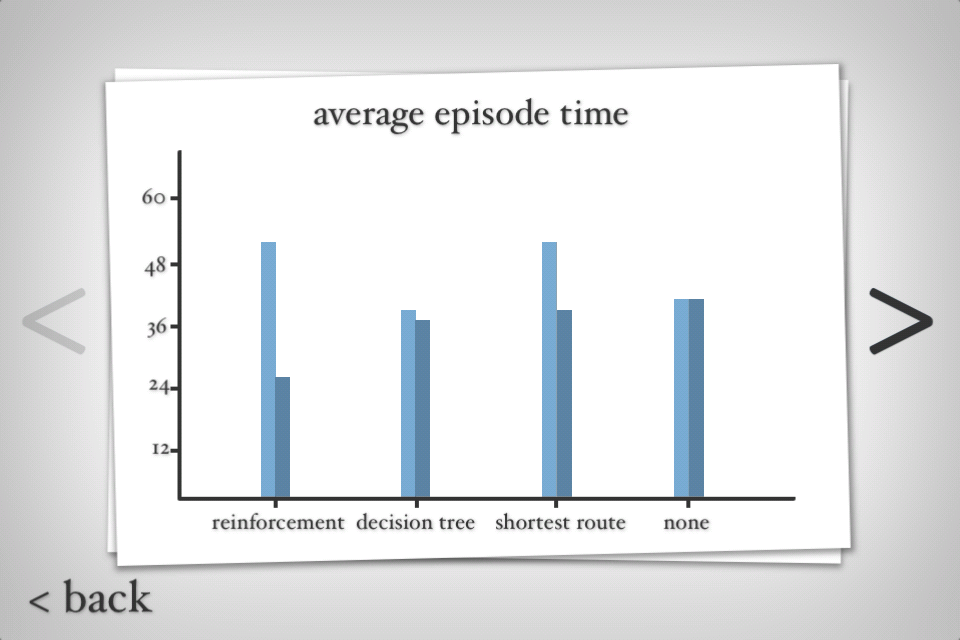
\includegraphics[width=85mm]{sources/images/GraphSlide}
    \caption{Game Stats Using the SlideViewer}
\end{figure}

\section{Problems Faced}
	
Fortunately, I didn't encounter any major issues when it came to implementing my learning. One fairly minor problem that I did come across was that I found it was possible for agents to get stuck in an `infinite decision loop'. After an agent had finished learning, it was possible for it to transition to a state whereby there was only one possible decision point (see Figure 14 for an example). If certain actions in this state led to certain death, then an agent could be forced to keep looping back and forth, which meant that the game couldn't be finished without the user prematurely quitting.

\begin{figure}[h!]
  \centering
    
\includegraphics[width=85mm]{sources/images/InfiniteLoop}
    \caption{An Example of a Possible `Infinite Decision Loop' State}
\end{figure}

The problem was being caused because I had programmed my agents to stop learning once the learning mode was over. My solution to this problem therefore was to allow the agents to continue to update the knowledgebase after the learning mode was complete. This worked because of the fact that I had applied a small negative reward to every action taken by the agent, meaning that were an agent caught in an infinite decision loop, the small negative rewards would build up and eventually filter to the previous states, meaning that agents would not fall into the same trap.
	
	
	
%
% New part
%

\part{Testing \& Evaluation}{This section presents the usability and learning testing I performed, the results that were obtained, and an analysis of the product's performance.}

\chapter{Testing \& Results}

In this section I present the results to my usability tests, in addition to the results from the AI testing. I initially planned to create some unit tests to test the functionality of my game. However, as the user-input was very limited, I didn't feel that this was necessary.

\section{Usability Testing and Error Checking}

As a result of my iterative design approach, I was regularly testing my game as I implemented new features and fixing any bugs as they arose. As I was working alone, this was the most appropriate method. For this reason, I didn't make as much use of bug tracking software as I would if I was working in a development team. However, I did make some use of Github's built in issue-tracking to record major errors, or errors I couldn't fix at the time of finding.

My game was designed as a test for machine learning in a game environment and as such, user interaction was always intended to be limited. Due to this, the usability tests which could be carried out were similarly limited; there was little other than basic user-interface testing which was needed.

One bug that was picked up during the usability tests that I wasn't able to solve was a problem with the game pausing. I found that when resuming the game, it was possible for agents to fall though the environment. This occurred if the game was paused while the agents were mid-way through transitioning to a lower level. I think the problem was with a `delay' method I used when agents use an umbrella or drop to a lower level, the problem being that the delay was cut short if the game was paused.

I came up with a partial solution to this problem, although the issue does still occur if there are many agents in the level. My solution was to change how I was pausing the game. To begin with, I was manually iterating through all of the objects in the game, and pausing them one by one. To try and fix the problem, I instead decided to use a function in Cocos2D's \emph{Director} class (the same method used by the engine when the user sends the app to the background by pressing the home button).


\section{AI Testing}

In addition to the usability tests, I also carried out extensive tests of my AI system. The primary aim of these tests being to check the effectiveness of the learning techniques, as well as to compare each technique against the others.



%
% New part
%

\chapter{Evaluation}

In this section, I provide analysis of my learning techniques and their effectiveness, as well as a more general evaluation of my project as a whole.

\section{Time Management}

When planning the development of my project and creating my project schedule, I initially planned to take a linear `waterfall' development approach \cite{Rerych:gb}. I planned to develop the game and AI components separately, conducting testing at the end of development. However, during development I took a more incremental approach; developing individual features and testing as I went along. This change in approach was partly due to the fact that I was unfamilar with developing in Objective-C

In terms of sticking to my initial schedule, I feel that the development ran fairly smoothly, albeit with a few slight changes to my initial plan. As testing was carried out incrementally, there was no final testing stage at the end of development. 

The biggest miscalculation with regards to my time-management and project schedule was that I failed to recognise just how much groundwork was needed to build the game component. Though I by no means expected the game development to be a trivial task, I wasn't prepared for the amount of work that was needed. This was exacerbated by the fact that I was also still getting to grips with Objective-C, and so my productivity wasn't as it could have been. However, although I slipped by a couple of weeks during the game development stage, I finished the AI component of the game under-schedule. Looking back at the volume of code that was needed to get the game running, it seems fairly obvious that I should have at least allocated an equal amount of time to both the game and AI components. As it happens, I still finished my project to schedule with some time to spare.

\section{Analysis of Machine Learning}

Overall, I think the the learning element of my system was very effective, with all learning types implemented showing an improvement over the agents with no learning. In this section, I provide some more in-depth analysis of each technique.

\subsection{Shortest Route Learning}

The shortest route technique is the most naive of those I implemented. This being said, it still provided a great improvement over the agents without learning, which was after all the ultimate goal. The main advantage to this method is that it is simple to implement, is quick and computationally cheap to function (there are no complex tree structures to search for example) and it yeilds effective results. 

However, this method also has some significant disadvantages. The biggest being the accuracy or indeed the optimality of the `optimal' routes it produces. The obvious flaw in this method being that the `optimum' route is completely dependant on the agent actually \emph{taking} the shortest route. Although this does not present a major problem with my levels, the greater the level size, the smaller the likelihood that the agent will discover the optimum route (or even any route at all). My results reveal that there were still appriximately $\frac{1}{5}$ of agents which were unable to find any safe path even in my small levels. This problem is only likely to increase with the size of the level. One of the biggest disadvantages to this method is that unsuccessful routes are disgarded and do not contribute to the knowledgebase, so are essentially a waste of time. 

This being said, I feel that there are a number of changes which could be made to this method which would greatly improve it. One possible enhancement which would greadly reduce the space complexity of the method is to remove the need to store each individual route. Instead, a simple check could be made at the end of each learning episode to determine whether the new route is an improvement over the previous route. This way, only the optimum route would need to be stored. This would also remove the need to iterate through a long list of routes after the agent's learning is complete. Another possible enhancement to this method is to implement a shared knowledgebase. This could take the form of a shared list of all routes, or as with my previous recommendation, be a shared copy of the optimum route so far. The benefit to using a shared knowledgebase has been proven in my Q-learning implementation; it greatly improves the efficiency and speed of learning. Another area which I feel that this method falls down on is in the comparison of different routes. In it's current state, my shortest route method simply takes the route which has the smallest number of moves (or actions). If there are multiple optimum routes, then the first route found is used. This route selection could be greatly improved by using some kind of weighting system similar to what was used in the decision tree method; whereby each route is given a `weight', determined by the number of tool uses in that route. This encourages the selection of routes with less tool uses. A final area in which I feel that this method could be improved is by implementing some way to build a `hybrid' route using the stored routes. This way, a truly optimum route could be found, even if the agent hadn't actually taken it.

\subsection{Decision Tree Learning}

Although I originally planned to implement decision tree learning, I didn't feel that my problem could be solved using classification, and so my tree method takes a slightly different approach. Unlike most decision tree learning methods which use classification techniques to learn, my decision tree implementation dynamically creates a map of the environment using a tree structure, and building a route from it. It takes a similar approach to the shortest route method but obviously using a more advanced method of storing the routes. However, it improves upon the storage space required by the shortest route method by only storing states once. One of the biggest advantages to this method over the shortest route is that even unsuccessful episodes contribute positively to the knowledgebase, and can be used later. Additionally, it improves over the shortest route method's route selection process by calculating `weightings' for the routes. This encourages the choice of routes with less tool uses. As with the shortest route method, it provides a considerable improvement over the agents with no learning. It also offers an improvement to the length of the optimum route when compared with the shortest route. 

However, my decision tree method also shares some of the pitfalls of the shortest route method. One such problem being the fact that it is similarly reliant on the agents discovering an optimal route whilst they are exploring the environment. As with shortest route, the chance of even completing the level successfully decreases as the level size grows, so relying soley on this is not advisable. This method is also more computationally expensive and slower than the shortest route method, as the tree must be exhaustively searched and an `optimum' route built. In addition to this, the method doesn't provide a great improvement over the shortest route method, which makes the extra computation time unjustifiable.

One improvement which could be made to improve this method could be to provide some more powerful route filtering to determine optimal routes. A simple way to do this is to incorporate the route's weighting into the its length; currently the algorithm only uses the weightings to compare two routes of the same length. This would produce `cheaper' routes than at present, as it would cause the system to choose routes which may be slighly longer, but don't use as many tools. Another improvement which could be made to this method is to introduce a shared knowledgebase. This would greatly increase the chance of an optimal route. I also think that a more efficient search method could be used in anticipation of the use of much larger levels. An heuristic algorithm such as A* would be appropriate.

\subsection{Reinforcement Learning}

Overall, my RL agents performed even better than expected, with the agents able to fairly quickly gather enough information to formulate an optimum policy. In addition, after a reasonable amount of episode, the method gave a 100\% survival rate which is as good as can be expected. A big advantage to this method is that every decision made by the agents contributes positively to the knowledgebase in a positive way; an agent dying is as helpful as if the agent had reached the exit, if not more so, as it teaches the agent where \emph{not} to go. In addition, the Q-learning algorithm is capable of functioning in much larger environments, given enough storage space. Another big advantage to this method is that it requires very little computation to build the optimum policy after the learning is complete, as the agent only needs to search through the actions currently avaliable to it for the current state; there is no need to search through vast knowledgebases, or build the complete route beforehand. For this reason, I feel that this method is particularly suited to a game environment, where high performance is paramount.

However, there are also a number of areas which let this method down. One problem being the amount of storage space required. The algorithm requires that every action/state combination tried by the agent needs to be stored. While this is not an issue in my game due to the small environments, this could cause problems in much larger environments - especially if using mobile hardware. Another problem with my implementation is that it never truly converges; the route taken by the agent is not necessarily the optimum route. The main cause for this being the amount of time given for the system to learn. As the method relies on a backwards propagation of rewards, it can take some time for said rewards to transfer the rewards to certain areas of the level. In the majority of machine learning systems, the algorithms are run for several thousand iterations, which gives it enough time to converge on a solution. With each learning episode in my game taking between 1 and 1.5 minutes, there is not enough time to allow the AI system to run for this many iterations. My addition of a shared knowledgebase greatly helped with this, as it meant that I was essentially `threading' the learning process using many agents to simultaneously contribute to the same knowledgebase. This greatly reduced the time required for an optimal solution to be found. 

Although my RL agents proved to be very effective, there are a few improvements which I would like to have made was I given more time. One such improvement being the addition of a variable learning rate. I discovered from my research that the general consensus is to begin the learning with a high learning rate, reducing it as time goes on, which has the effect of quicker learning early on, with more fine-tuning to the system later on. Using a variable learning rate would result in more accurate policies. However, I made a decision during the implementation stage to use a fixed rate for the simple reason that it would produce results much faster, which is key in a game environment; players don't have time to wait for hours for the AI to adjust. Another small enhancement I would like to make is to provide some way to save and load policies. Doing this and updating the same policies would allow the policies to converge, resulting in much more accuracy.

Test alternative reinforcement methods (bucket brigade, temporal difference) 

\section{General Areas For Enhancement}

Although I'm very pleased with the outcome of my project, given extra development time, there are a number of areas which I feel I would like to extend further.

The first and perhaps most obvious enhancement that I would make would be to extend the AI system to incorporate more learning types. Were I to do this, the next type that I would experiment with would be genetic algorithms, as I think that it lends itself quite well to the context of my game. Each individual agent could act as a gene, with only those agents with the most effective policies being chosen for `breeding'. The agents could spawn in waves representing a single generation of genes.

Another enhancement that I think it would be interesting to make would be to allow for multiple learning types to be used in a single game, with separate agents able to use different algorithms. It would be interesting to compare the performance of the methods in a single game. 

Something else which I'd like to implement would be some way for the agents to learn from each other - perhaps by `watching' (or being in the vicinity of) other agents. This wouldn't be as effective as using a shared knowledegbase, but it would create some more diverse behaviour among the agents, rather than every agent using the same route. While not necessarily appropriate to my problem area, it could definitely be useful in commercial games, where the AI agents need to appear realistic, by employing a diverse range of behaviour.

Another much simpler enhancement which I would like to make to my game would be to introduce much bigger levels. Although the agents show a definite improvement in their traversal of the level, I don't feel that using such small levels allows my system to fully demostrate its capabilities. I did initially look into creating levels which were several screen-widths wide, with the player able to scroll along the level. However due to the size restrictions of the iPhone screen, I later decided against this as I thought that it would be bad from a usability point of view, as the majority of the game level would be obscured to the player. It would perhaps be more appropriate to create a version of the game for a desktop computer.

A small criticism I have of my system is that it is very specific to the individual levels; the information learnt about one level is completely useless for another (a problem known as over-fitting). This being said, it is very difficult to design such a system, especially in a problem area such as mine, where it is very difficult to generalise. Additionally, The task of discovering n optimum route in an environment is very difficult to solve without over-fitting. A possible solution could be to develop the AI in two components: one using Q-learning to learn the policy for that individual level, and another (possibly a genetic algorithm) to learn more general rules. 

\section{Conclusion}

I am very happy with how my final system turned out. All of the learning types I implemented showed a significant improvement over the agents with no learning, which was my main goal. The reinforcement agents in particular are very effective in finding the optimum solution in a relatively limited number of learning episodes. Particularly so when utilising the shared knowledgebase. 

Learning aside, I was also very pleased with the core `game' component; especially given the fact that I had to create the artwork and character animations, and program the core game component myself. I feel that the final game is very robust, and serves well to demonstrate my AI system especially given the initial problems I encountered due to my inexperience of using Objective-C.

I felt I learnt a great deal carrying out this project. Aside from the knowledge of AI and machine learning gained, I also learnt a great deal about software and game development more generally. Having never developed a software product to completion, carrying out the initial design, specification through to the development and testing was invaluable. I found this project to be particularly useful from a game development point of view. Due to the fact that I was developing for mobile hardware, there were a number of considerations which I had to make such as the reuse of assets and other optimisation; issues which are often forgotten because of the powerful hardware at our disposal.

Most importantly of all, I feel that I suitably demonstrated that it is not only possible, but computationally feasible with today's technology to implement machine learning techniques in games. Even more so given the fact that I did so on a mobile device (although I accept that not all mobile games have the same amount of processor time to devote to the AI). Such techniques could have many possible applications in games to create much more `intelligent' AI systems which are capable of dynamically modifying their behaviour to adapt to the player. Given that machine learning techniques have been shown to be effective in commercial games (Lionhead's Black \& White is a good example), it is surprising to me that more developers haven't taken up the mantle and implemented similar techniques in their own games. Such techniques could be applied to virtually any game genre, from enemy commanders in a real-time strategy war game, to the AI-controlled players in a football game, to enemy characters in a platform game. This, in addition to the increase in importance given to the AI in the form of more processor time, and programmers dedicated to AI development suggest to me that such techniques are likely to become more widespread in the near future. 


%
% New part 
%

\part{Appendices}{}

	\appendix
	
	%\chapter{Code Listings}

	\chapter{Project Log}
	
A day-by-day work diary kept by you as the project is carried out. A log which has evidently been manufactured to be handed in rather than having been properly kept will result in a lower grade.

	\chapter{Git Log}


	
%
% References
%

\singlespace

\newpage
\addcontentsline{toc}{part}{Bibliography}
\bibliographystyle{abbrv}
\bibliography{Cogito}

\end{document}
